% !TEX program = xelatex
\documentclass[withoutpreface]{cumcmthesis}

\usepackage{tikz}
\usepackage{pythonhighlight}
\usetikzlibrary{positioning, arrows.meta, calc, shapes.geometric}
\captionsetup{font=small}
\newtheorem{proposition}{命题}
% 图题下方的补充说明：用灰色小字与标题分开，且区别于正文
\usepackage{xcolor}
\definecolor{noteGray}{gray}{0.45}
\newcommand{\figexp}[1]{\par\vspace{3pt}{\footnotesize\color{noteGray} 说明：#1}\par\vspace{5pt}}
% 放宽浮动体放置限制，减少图表造成的整页空白
\renewcommand{\topfraction}{0.92}
\renewcommand{\bottomfraction}{0.85}
\renewcommand{\textfraction}{0.04}
\renewcommand{\floatpagefraction}{0.75}
\setlength{\floatsep}{8pt plus 2pt minus 4pt}
\setlength{\textfloatsep}{10pt plus 2pt minus 4pt}
\setlength{\intextsep}{8pt plus 2pt minus 4pt}

\title{基于嵌套联合优化与射线追踪的FAST主动反射面调节模型}

\begin{document}

\maketitle

\begin{abstract}
FAST主动反射面的形状调节，本质是在促动器行程与索长变化等紧约束下，用离散刚性面板拼接的可控曲面逼近观测方向决定的理想旋转抛物面。本文以基准球面球心$C$为原点建立坐标系，以焦距$p$为外层变量、节点径向伸缩量$\boldsymbol{\delta}$为内层变量建立\textbf{嵌套联合优化模型}，并以\textbf{矢量反射定律}与\textbf{投影面积加权}的射线追踪评估调节效果，形成``理想抛物面确定—反射面调节—接收比评估''的完整建模链条。

\textbf{针对问题一}，在天体位于基准球面正上方（$\alpha=0^{\circ}$、$\beta=90^{\circ}$）时确定理想抛物面。先由焦面半径差$0.466R$确定馈源舱位置，再由抛物面定义推导以焦距$p$为唯一参数的一般方程。求解前证明关键事实：直接取节点径向与抛物面交点为目标时，相邻索长最大相对变化达$0.12809\%$，远超$0.07\%$限值，即\textbf{理想交点解不可行}，$p$与$\boldsymbol{\delta}$必须联合优化。外层在$[139.9,\,140.9]\,\mathrm{m}$内搜索$p$，内层以``罚函数$+$多顺序坐标下降''的\textbf{混合多起点策略}求解非凸二次约束规划，求得$p^{*}=140.3773\,\mathrm{m}$，理想抛物面$x^{2}+y^{2}=561.5092\,(z+300.7909)$，$706$个口径内节点贴合残差均方根$46.3\,\mathrm{mm}$，索长最大相对变化$0.06997\%$，全部约束满足。

\textbf{针对问题二}（$\alpha=36.795^{\circ}$、$\beta=78.169^{\circ}$），将同一框架推广到一般观测方向，求得$p^{*}=140.3743\,\mathrm{m}$（与问题一仅差$3\,\mathrm{mm}$），理想抛物面顶点$V(-49.3837,\,-36.9370,\,-294.3982)\,\mathrm{m}$。针对``尽量贴近''未给定度量的问题，从节点、面板中心与整块面板积分三个层面提出三种方案，逐一实现并统一指标比较：三者最优焦距完全一致；方案二、三的面板精度仅改善$2.0\%$与$1.1\%$，节点精度反而下降约$1\%$、耗时增加约$40\%$，根源在于$0.07\%$索长约束将可行域压缩为狭窄``管道''。故采用\textbf{方案一}：$692$个口径内节点残差$51.5\,\mathrm{mm}$，伸缩量$[-0.2516,\,0.2142]\,\mathrm{m}$，结果按附件4格式存入\texttt{result.xlsx}。

\textbf{针对问题三}，建立基于\textbf{面板球心反演}与\textbf{射线追踪}的接收比模型：先由调节后三顶点反演各面板球心，得精确法向$N(M)=(M-\mathbf{O}_k)/R$；再由矢量反射定律求反射线与接收平面的交点$Q$，以$|Q-P|\le0.5\,\mathrm{m}$判接收，按投影面积加权求接收比。$1474$块面板、每块$210$点参与追迹，覆盖率$99.98\%$。计算得\textbf{调节后接收比$0.3407$，基准球面仅$0.0528$，提升$6.5$倍}；对理想抛物面直接追迹得$1.000000$，验证了判据与实现的自洽性。

最后，对\texttt{result.xlsx}所载方案执行六项独立校核\textbf{全部通过}；采样阶数$m=10\to30$时接收比波动不足$0.6\%$，数值收敛。焦距敏感性分析发现\textbf{贴合残差最小的焦距（$140.3743\,\mathrm{m}$）与接收比最大的焦距（约$140.45\,\mathrm{m}$）并不重合}——接收比主要惩罚导致光线偏折的倾斜误差，对整体径向平移的``活塞''误差不敏感。按题面``尽量贴近''的要求，本文采用\textbf{贴合优先准则}；若以接收效果为先，接收比可再提升约$45\%$。

\keywords{FAST主动反射面；嵌套联合优化；混合多起点坐标下降；矢量反射定律；射线追踪；接收比}
\end{abstract}

% ==================== 问题重述 ====================
\section{问题重述}

\subsection{问题背景}

中国天眼——500米口径球面射电望远镜（Five-hundred-meter Aperture Spherical radio Telescope，简称FAST），是我国自主建造的目前世界上单口径最大、灵敏度最高的射电望远镜\cite{nan2006,nan2011}。其\textbf{主动反射面}由主索网、反射面板、下拉索与\textbf{促动器}等构成：主索网按短程线三角网格布置并支承反射面板，每个主索节点经一根下拉索与地表促动器相连，促动器沿基准球面径向伸缩即可牵引节点变位，从而改变反射面形状。

主动反射面有\textbf{基准态}与\textbf{工作态}两种状态：基准态为半径约$300\,\mathrm{m}$、口径$500\,\mathrm{m}$的球面（\textbf{基准球面}，球心$C$）；工作态则被调节为口径$300\,\mathrm{m}$的近似旋转抛物面。馈源舱接收平面中心只能在与基准球面同心、半径差为$0.466R$的\textbf{焦面}上移动，其\textbf{有效接收区域}为直径$1\,\mathrm{m}$的中心圆盘。当观测方向为天体目标$S$时，\textbf{馈源舱}中心移至直线$SC$与焦面的交点$P$，并通过调节部分反射面板形成以$SC$为对称轴、$P$为焦点的近似旋转抛物面，将平行入射的电磁波汇聚至馈源舱。本赛题的\textbf{核心任务}，即在此调节机制约束下确定\textbf{理想抛物面}，并调节促动器的径向伸缩量使反射面尽量贴近该理想抛物面。观测剖面如图~\ref{fig:fast_profile}所示。

\begin{figure}[htbp]
    \centering
    \includegraphics[width=0.56\textwidth]{../figures/FAST_cross-sectional_schematic.png}
    \caption{FAST观测剖面示意图} \label{fig:fast_profile}
\end{figure}

\subsection{问题提出}

根据上述背景及附件所给参数，本文需要建立模型解决以下三个问题：

\textbf{问题一}：当待观测天体$S$位于基准球面正上方，即方位角$\alpha=0^{\circ}$、仰角$\beta=90^{\circ}$时，结合考虑反射面板调节因素，确定理想抛物面。

\textbf{问题二}：当待观测天体$S$位于$\alpha=36.795^{\circ}$、$\beta=78.169^{\circ}$时，确定理想抛物面；建立反射面板调节模型，调节相关促动器的伸缩量，使反射面尽量贴近该理想抛物面。将理想抛物面的顶点坐标，以及调节后反射面$300\,\mathrm{m}$口径内的主索节点编号、位置坐标、各促动器的伸缩量等结果，按附件4规定的格式保存在\texttt{result.xlsx}文件中。

\textbf{问题三}：基于第2问的反射面调节方案，计算调节后馈源舱的接收比，即馈源舱有效区域接收到的反射信号与$300\,\mathrm{m}$口径内反射面的反射信号之比，并与基准反射球面的接收比作比较。

% ==================== 问题分析 ====================
\section{问题分析}

\subsection{问题一分析}

问题一要求在天体$S$位于基准球面正上方（$\alpha=0^{\circ}$，$\beta=90^{\circ}$）时确定理想抛物面。此时视线$CS$沿$z$轴正方向，抛物面对称轴即$z$轴，馈源舱位于$z$轴上焦面与直线$SC$的交点处。需要先由焦面半径$0.534R$确定焦点坐标，再由抛物面的几何定义推导出以\textbf{焦距}$p$为参数的\textbf{一般方程}，此时$p$尚为待定参数。

确定$p$的准则是本题的难点：若仅要求抛物面在几何上通过馈源舱焦点，$p$仍有一个自由度的选择余地；题面要求``结合考虑反射面板调节因素''，故$p$的选取必须使调节后的反射面在约束下尽可能贴近该抛物面。本文首先验证一个关键事实：直接取节点径向与抛物面交点作为目标（\textbf{``理想交点解''}）时，相邻索长最大相对变化达$0.12809\%$，超过$0.07\%$限值，即理想交点解不可行。因此$p$与节点伸缩量$\boldsymbol{\delta}$必须联合优化——外层以$p$为决策变量、以约束下方案的贴合残差为目标，内层在促动器行程与索长变化约束下求最贴近理想交点的可行伸缩量。

\subsection{问题二分析}

问题二要求在$\alpha=36.795^{\circ}$、$\beta=78.169^{\circ}$时确定理想抛物面，并建立反射面板调节模型。与问题一相比有\textbf{两点扩展}：观测轴不再与坐标轴重合，抛物面一般方程不再退化为关于$z$轴的旋转曲面形式，须直接使用一般方程；且需给出可执行的调节方案并按指定格式提交。

关于``尽量贴近''这一表述，题面未给出明确的度量方式，本文从节点、面板中心与整块面板三个层面理解该要求，逐一建模实现：（i）仅要求主索节点（面板顶点）贴合理想抛物面；（ii）要求每块反射面板的中心点贴合；（iii）要求整块面板在其所占区域内整体贴合。三者分别导出不同的目标函数，本文通过统一指标的实验比较作出选择，而非先验地取其一。此外，反射面板为\textbf{刚性球面片}，调节后三顶点不再共处于以$C$为球心的球面上，每块面板都有自己独立的球心，因此评价``面板中心''或``整块面板''的贴合程度前必须先反演该面板的球心，这是问题二特有的一个几何子问题。

\subsection{问题三分析}

问题三要求基于问题二的调节方案计算馈源舱的\textbf{接收比}，即有效区域接收到的反射信号与$300\,\mathrm{m}$口径内反射信号之比。其一，调节后的反射面由$4300$块刚性球面片拼接而成，每块仍为半径$R$的球面的一部分但球心各不相同；若简单地以$M/|M|$近似法向，将完全丢失面板变位带来的法向偏转，接收比计算会失去意义，故必须先\textbf{反演各面板球心}得到$N(M)=(M-\mathbf{O}_k)/R$。其二，由\textbf{矢量反射定律}求反射线方向，与过焦点$P$、垂直于观测轴$\mathbf{n}$的接收平面求交得落点$Q$，以$|Q-P|\le0.5\,\mathrm{m}$判接收；该判据在理想抛物面上应处处成立（$Q\equiv P$），这提供了模型自洽性检验的途径。其三，入射为平行光，面元$\mathrm{d}S$承接的功率正比于其投影面积$|N\cdot\mathbf{n}|\,\mathrm{d}S$，故接收比应按\textbf{投影面积加权}而非按实际面积加权。最后对基准反射球面执行同一套计算作为对照，并检验采样收敛性与口径覆盖率。

\subsection{总体技术路线}\label{sec:tech}

综合以上分析，本文的技术路线如图~\ref{fig:flowchart}所示。三个问题共用同一套几何底座（坐标系、观测轴、焦点、抛物面一般方程、径向求交），问题一在其上叠加\textbf{嵌套联合优化}以确定焦距；问题二把同一框架推广到一般观测方向并比较三种\textbf{拟合优度方案}；问题三把几何结果通过\textbf{射线追踪}转换为物理指标。这三者首尾相接，前一问的输出即后一问的输入，保证了全篇结果的\textbf{一致性}。

\begin{figure}[htbp]
\centering
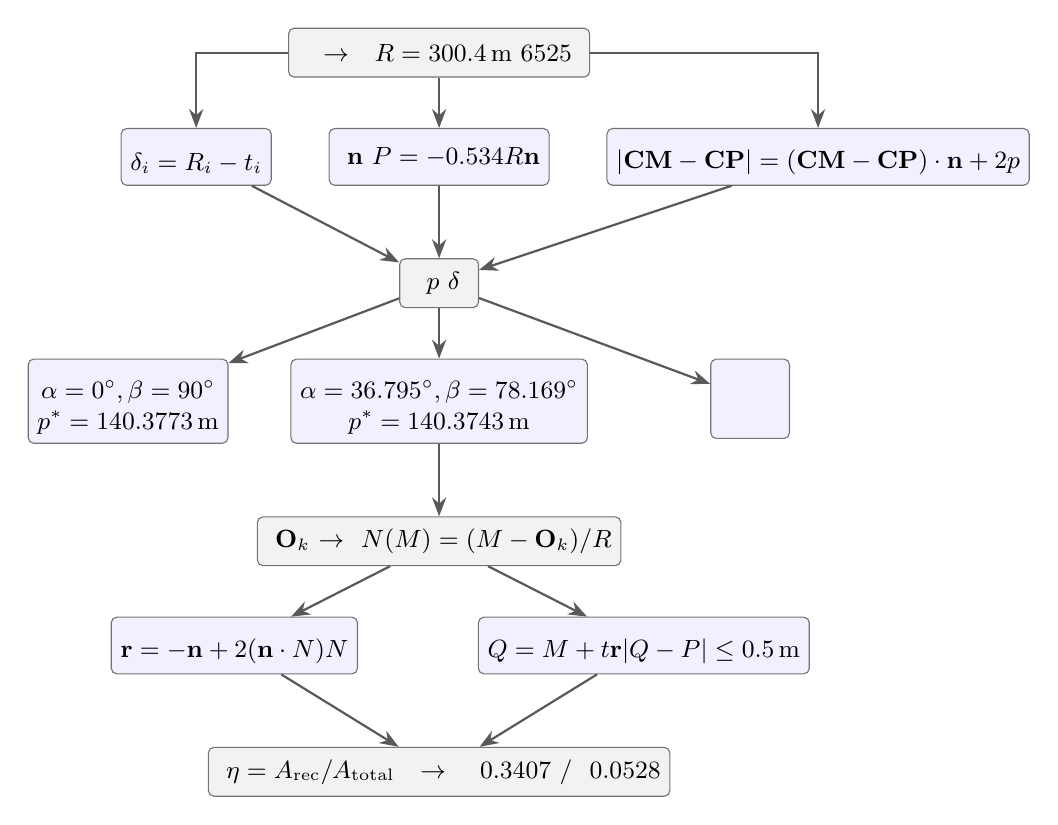
\begin{tikzpicture}[
    node distance=0.62cm and 0.5cm,
    box/.style={rectangle, draw=black!55, fill=blue!6, rounded corners=2pt,
                minimum width=1cm, minimum height=0.72cm, align=center, font=\small},
    bbox/.style={rectangle, draw=black!55, fill=gray!10, rounded corners=2pt,
                 minimum width=1cm, minimum height=0.62cm, align=center, font=\small},
    io/.style={rectangle, draw=black!55, fill=green!7, rounded corners=2pt,
               minimum width=1cm, minimum height=0.72cm, align=center, font=\small},
    arr/.style={-{Stealth[length=2.4mm]}, thick, draw=black!65}
]
\node[bbox] (s0) {节点坐标、邻接关系、面板构成\quad$\rightarrow$\quad $R=300.4\,\mathrm{m}$、索网边 $6525$ 条};

\node[box, below=of s0, yshift=-0.02cm] (s1) {观测轴 $\mathbf{n}$、焦点 $P=-0.534R\mathbf{n}$};
\node[box, right=0.72cm of s1] (s2) {理想抛物面一般方程\\$|\mathbf{CM}-\mathbf{CP}|=(\mathbf{CM}-\mathbf{CP})\cdot\mathbf{n}+2p$};
\node[box, left=0.72cm of s1] (s3) {径向求交：二次方程求根\\$\delta_i=R_i-t_i$};

\node[bbox, below=of s1, yshift=-0.3cm] (s4) {嵌套联合优化：外层一维搜索 $p$，内层混合多起点求约束下最贴近理想交点的可行 $\boldsymbol{\delta}$};

\node[box, below=of s4, yshift=-0.02cm, xshift=-3.95cm] (s5) {问题一\\$\alpha=0^\circ,\beta=90^\circ$\\$p^*=140.3773\,\mathrm{m}$};
\node[box, below=of s4, yshift=-0.02cm] (s6) {问题二\\$\alpha=36.795^\circ,\beta=78.169^\circ$\\$p^*=140.3743\,\mathrm{m}$};
\node[box, below=of s4, yshift=-0.02cm, xshift=3.95cm] (s7) {三种拟合优度方案\\统一指标比较\\选定方案一};

\node[bbox, below=of s6, yshift=-0.3cm] (s8) {面板球心反演 $\mathbf{O}_k$ $\rightarrow$ 精确法向 $N(M)=(M-\mathbf{O}_k)/R$};

\node[box, below=of s8, yshift=-0.02cm, xshift=-2.6cm] (s9) {矢量反射定律\\$\mathbf{r}=-\mathbf{n}+2(\mathbf{n}\cdot N)N$};
\node[box, below=of s8, yshift=-0.02cm, xshift=2.6cm] (s10) {接收平面求交\\$Q=M+t\mathbf{r}$，$|Q-P|\le0.5\,\mathrm{m}$};

\node[bbox, below=of s9, yshift=-0.3cm, xshift=2.6cm] (s11) {投影面积加权 $\eta=A_{\mathrm{rec}}/A_{\mathrm{total}}$\quad$\rightarrow$\quad 调节后 $0.3407$ / 基准 $0.0528$};

\draw[arr] (s0) -- (s1);
\draw[arr] (s0.east) -| (s2.north);
\draw[arr] (s0.west) -| (s3.north);
\draw[arr] (s1) -- (s4);
\draw[arr] (s2) -- (s4);
\draw[arr] (s3) -- (s4);
\draw[arr] (s4) -- (s5);
\draw[arr] (s4) -- (s6);
\draw[arr] (s4) -- (s7);
\draw[arr] (s6) -- (s8);
\draw[arr] (s8) -- (s9);
\draw[arr] (s8) -- (s10);
\draw[arr] (s9) -- (s11);
\draw[arr] (s10) -- (s11);
\end{tikzpicture}
\caption{本文总体技术路线}
\figexp{灰色横条为三问共用的几何底座与最终输出，蓝色框为各环节的核心模型。}
\label{fig:flowchart}
\end{figure}

% ==================== 模型假设 ====================
\section{模型假设与合理性说明}

\begin{description}
\item[1. 基准球面的理想性] 全部主索节点位于以$C$为球心、半径$R=300.4000\,\mathrm{m}$的球面上。\textit{依据}：节点模长标准差仅$0.216\,\mathrm{mm}$，相对偏离$10^{-6}$量级，远小于本文讨论的形变尺度。

\item[2. 面板的刚性] 反射面板为理想刚性球面片，形状由三顶点（主索节点）唯一决定，调节中无弯曲与热变形。\textit{依据}：面板为铝合金背架结构，面内刚度远大于索网变形尺度，题面亦以此为设定。

\item[3. 促动器的径向行程] 促动器沿基准球面径向伸缩，行程限幅$\pm0.6\,\mathrm{m}$，调节后$P_i'=P_i+\delta_i\,\mathbf{e}_i$。\textit{依据}：题面给出限幅并说明下拉索沿径向牵引。

\item[4. 索长不变的近似] 调节中主索长近似不变，以相邻节点间距相对变化不超过$0.07\%$刻画。\textit{依据}：题面给出该限值；主索为高强钢索，弹性伸长远小于限值对应的$7.97\,\mathrm{mm}$。

\item[5. 几何光学近似] 电磁波沿直线传播，反射遵循矢量反射定律\cite{bornwolf}，忽略衍射与多次反射。\textit{依据}：工作波长厘米至米量级，$\lambda/D\ll1$；缝隙仅占口径$0.02\%$。

\item[6. 入射光的平行性] 来自天体的电磁波为平行于观测轴$\mathbf{n}$的平行光，口径内光强均匀。\textit{依据}：天体距离远超望远镜尺度，入射可视为平面波。

\item[7. 仅调节照明区] 仅$300\,\mathrm{m}$口径内节点参与调节，口径外伸缩量取$0$。\textit{依据}：题面要求提交口径内节点结果；索长约束仍纳入跨接边以避免边界违约。
\end{description}

% ==================== 符号说明 ====================
\section{符号说明}

\begin{longtable}{c p{4.2cm} c | c p{4.2cm} c}
\toprule
符号 & 说明 & 单位 & 符号 & 说明 & 单位 \\
\midrule
\endfirsthead
\toprule
符号 & 说明 & 单位 & 符号 & 说明 & 单位 \\
\midrule
\endhead
\bottomrule
\endfoot
\bottomrule
\endlastfoot
$R$ & 基准球面半径（$=300.4000$） & $\mathrm{m}$ & $p$（$p^*$） & 抛物面焦距（最优值） & $\mathrm{m}$ \\
$C$ & 基准球面球心（坐标原点） & --- & $\mathbf{n}$ & 观测轴（抛物面轴）单位向量 & --- \\
$\alpha,\beta$ & 天体方位角、仰角 & $^{\circ}$ & $a,b,c$ & $\mathbf{n}$的三个分量 & --- \\
$P$ & 馈源舱（抛物面焦点） & --- & $V$ & 抛物面顶点 & --- \\
$M$ & 抛物面/镜面上任意一点 & $\mathrm{m}$ & $t$ & 径向与抛物面交点的距离 & $\mathrm{m}$ \\
$A_i$ & $\mathbf{u}_i\cdot\mathbf{n}$（方向余弦） & --- & $R_i$ & 节点$i$到球心距离 & $\mathrm{m}$ \\
$\hat{\delta}_i$ & 理想交点伸缩量 & $\mathrm{m}$ & $\delta_i$（$\delta_i^*$） & 可行伸缩量（内层最优解） & $\mathrm{m}$ \\
$\mathcal{I}$ & 口径内节点集合 & --- & $E$ & 参与索长约束的边集合 & --- \\
$\varepsilon$ & 索长相对变化限值 $0.07\%$ & --- & $\Delta_{\max}$ & 促动器行程限幅 $0.6$ & $\mathrm{m}$ \\
$\mathrm{RMS}(p)$ & 约束下贴合残差均方根 & $\mathrm{m}$ & $\lambda$ & 罚因子 & --- \\
$\mathbf{O}_k$ & 第$k$块面板的球心 & $\mathrm{m}$ & $\mathbf{G}_k$ & 第$k$块面板的中心点 & $\mathrm{m}$ \\
$N(M)$ & $M$处的单位法向量 & --- & $\mathbf{r}$ & 反射线方向向量 & --- \\
$Q$ & 反射光在接收平面上的落点 & $\mathrm{m}$ & $x_f(M)$ & 反射点横向偏移$|Q-P|$ & $\mathrm{m}$ \\
$A_{\mathrm{rec}}$ & 被接收的投影面积 & $\mathrm{m}^2$ & $A_{\mathrm{total}}$ & 总投影面积 & $\mathrm{m}^2$ \\
$\eta$ & 接收比 & --- & $m$ & 面板采样阶数 & --- \\
\bottomrule
\end{longtable}

% ==================== 模型准备 ====================
\section{模型准备：坐标系与关键几何量}

本节建立三问共用的\textbf{几何底座}。除最终代入的具体角度外，本节所有结论对任意方位角$\alpha$与仰角$\beta$均成立。

\subsection{坐标系与观测轴}

取基准球面球心$C$为坐标原点，建立三维直角坐标系$Oxyz$。设天体方位角为$\alpha$、仰角为$\beta$，则由球坐标定义，由$C$指向天体$S$的观测轴线单位向量为
\begin{equation}\label{eq:axis}
\mathbf{n}=(a,b,c)=(\cos\beta\cos\alpha,\;\cos\beta\sin\alpha,\;\sin\beta)
\end{equation}

易验证$|\mathbf{n}|^{2}=\cos^{2}\beta(\cos^{2}\alpha+\sin^{2}\alpha)+\sin^{2}\beta=1$。以问题二为例，$\alpha=36.795^{\circ}$、$\beta=78.169^{\circ}$代入得$\mathbf{n}=(0.164181,\,0.122801,\,0.978757)$。

\subsection{焦点与顶点的定位}

馈源舱（即工作抛物面的焦点）记为$P$，它位于与基准球面同心、半径差为$0.466R$的焦面上。因焦面半径$=R-0.466R=0.534R$，且$P$在观测轴与焦面的交点上（位于$C$的背向$S$一侧），故焦点位置矢量为
\begin{equation}\label{eq:focus}
\overrightarrow{CP}=-0.534R\,\mathbf{n}
\end{equation}

即焦点$P$到球心$C$的距离恒为$0.534R=160.4136\,\mathrm{m}$，与观测方向无关，仅沿轴$\mathbf{n}$的反方向变化。

设抛物面顶点为$V$、\textbf{焦距}为$p$。顶点在轴上位于焦点沿$-\mathbf{n}$方向、距焦点$p$处：
\begin{equation}\label{eq:vertex}
V=P-p\,\mathbf{n}=-(0.534R+p)\,\mathbf{n}
\end{equation}

由式~\eqref{eq:vertex}，抛物面一经确定，其顶点到球心$C$的距离即为$0.534R+p$，这是后文判断抛物面与基准球面相对位置的直接依据。

\subsection{理想抛物面的一般方程}

设抛物面上任一点为$M(x,y,z)$，$\mathbf{CM}=(x,y,z)$为其位置矢量。由\textbf{抛物面的定义}——点到焦点的距离等于该点沿轴线方向到准线的距离——有
\begin{equation}\label{eq:def}
\left|\mathbf{CM}-\mathbf{CP}\right|=\left(\mathbf{CM}-\mathbf{CP}\right)\cdot\mathbf{n}+2p
\end{equation}

其几何意义如图~\ref{fig:paraboloid_def}所示：右端第一项$(\mathbf{CM}-\mathbf{CP})\cdot\mathbf{n}$是$M$相对焦点沿轴向的有向距离，加上$2p$即$M$到准线的距离。

\begin{figure}[htbp]
    \centering
    \includegraphics[width=0.54\textwidth]{../figures/抛物面定义.pdf}
    \caption{抛物面几何定义示意图} \label{fig:paraboloid_def}
\end{figure}

将$\mathbf{CM}=(x,y,z)$与式~\eqref{eq:focus}代入，注意到
\begin{equation}
\left(\mathbf{CM}-\mathbf{CP}\right)\cdot\mathbf{n}=ax+by+cz+0.534R\left(a^{2}+b^{2}+c^{2}\right)=ax+by+cz+0.534R
\end{equation}

（利用了$|\mathbf{n}|=1$），对式~\eqref{eq:def}两边平方并整理，得
\begin{equation}\label{eq:paraboloid}
(x+0.534Ra)^{2}+(y+0.534Rb)^{2}+(z+0.534Rc)^{2}=(ax+by+cz+0.534R+2p)^{2}
\end{equation}

式~\eqref{eq:paraboloid}即为一般情形下理想抛物面的隐式方程。它由焦距$p$唯一确定：给定$p$后，抛物面的轴线、焦点、顶点全部随之确定。因此\textbf{``确定理想抛物面''在本模型中即等价于``确定焦距$p$''}。$p$的确定准则见第~\ref{sec:nested}节。

\subsection{径向求交与理想伸缩量}\label{sec:radial}

理想抛物面确定后，各主索节点应调节到什么位置？由于促动器只能沿基准球面\textbf{径向}牵引节点，最自然的做法是：让节点沿其自身的\textbf{径向}移动到与理想抛物面的交点处。记节点$i$的径向单位向量$\mathbf{u}_i$、到球心距离$R_i$，交点$M_i=t_i\mathbf{u}_i$，代入式~\eqref{eq:paraboloid}并整理，得到关于$t_i$的二次方程
\begin{equation}\label{eq:quad}
(1-A_i^{2})\,t_i^{2}-4pA_i\,t_i+4p(B-p)=0,\qquad A_i=\mathbf{u}_i\cdot\mathbf{n},\quad B=-0.534R
\end{equation}

其判别式为
\begin{equation}\label{eq:disc}
\Delta_i=16A_i^{2}p^{2}-16(1-A_i^{2})p(B-p)=16p\bigl[p-B(1-A_i^{2})\bigr]=16p\bigl[p+0.534R(1-A_i^{2})\bigr]
\end{equation}

因$p>0$、$R>0$、$1-A_i^{2}\ge0$，恒有$\Delta_i>0$，\textbf{径向交点总存在且唯一}。取使$t_i>0$且$t_i\approx R_i$的根
\begin{equation}\label{eq:root}
t_i=\frac{4pA_i+\sqrt{\Delta_i}}{2(1-A_i^{2})}\quad(1-A_i^{2}>10^{-12}),\qquad t_i=\frac{B-p}{A_i}\quad(A_i=\pm1)
\end{equation}

定义节点$i$的\textbf{理想交点伸缩量}（向球心为正）
\begin{equation}\label{eq:delta_hat}
\hat{\delta}_i=R_i-t_i
\end{equation}

$\hat{\delta}_i>0$表示该节点需沿径向朝球心内缩，$\hat{\delta}_i<0$表示需向外推出。

为检验式~\eqref{eq:quad}--\eqref{eq:delta_hat}的正确性并展示中间计算过程，表~\ref{tab:radial_demo}列出问题二方向下$6$个代表性节点（按到观测轴距离$d$由中心向边缘选取）的各中间量。

\begin{longtable}{c r r r r r}
\caption{径向求交的中间计算量示例（问题二，$p=140.3743\,\mathrm{m}$，$B=-0.534R=-160.413606\,\mathrm{m}$）} \label{tab:radial_demo} \\
\toprule
节点 & $d\,(\mathrm{m})$ & $A_i=\mathbf{u}_i\cdot\mathbf{n}$ & $1-A_i^{2}$ & $\Delta_i\;(\mathrm{m}^4)$ & $t_i\;(\mathrm{m})$ \\
\midrule
\endfirsthead
\toprule
节点 & $d\,(\mathrm{m})$ & $A_i$ & $1-A_i^{2}$ & $\Delta_i$ & $t_i\;(\mathrm{m})$ \\
\midrule
\endhead
\bottomrule
\endfoot
\bottomrule
\endlastfoot
D27 & $0.001$ & $-1.000000$ & $0.000000$ & $315279.25$ & $300.787628$ \\
E17 & $29.927$ & $-0.995025$ & $0.009925$ & $318855.17$ & $300.685695$ \\
D59 & $59.859$ & $-0.979946$ & $0.039707$ & $329585.04$ & $300.430216$ \\
D120 & $89.891$ & $-0.954179$ & $0.089542$ & $347540.26$ & $300.173224$ \\
D204 & $119.977$ & $-0.916780$ & $0.159514$ & $372750.10$ & $300.171118$ \\
D249 & $145.053$ & $-0.875694$ & $0.233160$ & $399283.69$ & $300.628844$ \\
\midrule
\multicolumn{6}{p{13.2cm}}{\small 注：$d$为节点到观测轴的距离。由$t_i$即得$\hat{\delta}_i=R_i-t_i$，依次为 $-387.57$、$-285.72$、$-30.24$、$+226.81$、$+228.67$、$-229.05\;\mathrm{mm}$，呈``中心外推—中环内缩—边缘再外推''的\textbf{三段式}而非简单的抛物线形，源于球面与抛物面的二阶曲率差异。}\\
\bottomrule
\end{longtable}

需要说明的是，$\hat{\delta}_i$只是``理想''目标，未必可行。表~\ref{tab:radial_demo}已经显示出问题的端倪：$\hat{\delta}_i$的幅度达$200\sim390\,\mathrm{mm}$，而$0.07\%$的\textbf{索长约束}只允许相邻节点产生约$8\,\mathrm{mm}$的相对径向位移差。两者相差近两个数量级，这决定了后文调节模型的\textbf{基本形态}。

% ==================== 问题一 ====================
\section{问题一：理想抛物面与调节方案的联合确定}\label{sec:nested}

\subsection{理想交点解不可行性的验证}

在建立优化模型之前，先验证一个决定模型形态的\textbf{关键事实}：直接取$\delta_i=\hat{\delta}_i$的``理想交点解''是否满足调节约束。

由数据预处理，索长均值$11.3906\,\mathrm{m}$，$0.07\%$限值折算为$7.97\,\mathrm{mm}$。而在问题一情形（$\alpha=0^{\circ}$、$\beta=90^{\circ}$）下，理想交点伸缩量的范围为$[-390.92,\,277.11]\,\mathrm{mm}$，其沿径向的空间变化远超$8\,\mathrm{mm}$的索长变化限值。数值实验证实了这一判断：直接令$\delta_i=\hat{\delta}_i$时，$2205$条相关索的最大相对长度变化为
\begin{equation}
\max_{e\in E}\frac{\bigl|\,|P_i'-P_j'|-|P_i-P_j|\,\bigr|}{|P_i-P_j|}=0.12809\%>0.07\%
\end{equation}

超出限值近一倍，\textbf{理想交点解不可行}。这意味着``先按几何确定抛物面、再把节点移到交点上''的\textbf{两步走}思路在本问题中根本走不通，抛物面的确定与节点的调节必须\textbf{作为一个整体求解}。

\subsection{嵌套联合优化模型}

记$\mathcal{I}$为$300\,\mathrm{m}$口径内的主索节点集合（到观测轴距离$\le150\,\mathrm{m}$），$E$为与该集合相关联的索的集合（含一端在口径内的跨接边），$\varepsilon=0.07\%$为索长相对变化限值，$\Delta_{\max}=0.6\,\mathrm{m}$为促动器行程限幅。建立如下两层结构。

\textbf{内层（给定$p$）：求约束下最贴近理想交点的可行伸缩量。}决策变量为$\boldsymbol{\delta}=(\delta_i)_{i\in\mathcal{I}}$，目标为最小化相对理想交点的偏差平方和：
\begin{subequations}\label{eq:inner}
\begin{align}
\min_{\boldsymbol{\delta}}\quad & f(\boldsymbol{\delta};p)=\sum_{i\in\mathcal{I}}\bigl(\delta_i-\hat{\delta}_i(p)\bigr)^{2}\label{eq:inner_obj}\\
\text{s.t.}\quad & |\delta_i|\le\Delta_{\max}, && i\in\mathcal{I}\label{eq:inner_c1}\\
& \Bigl|\,|P_i'-P_j'|-|P_i-P_j|\,\Bigr|\le\varepsilon\,|P_i-P_j|, && (i,j)\in E\label{eq:inner_c2}
\end{align}
\end{subequations}

其中$P_i'=P_i+\delta_i\mathbf{e}_i$为调节后节点位置。约束~\eqref{eq:inner_c2}中，由于径向移动不改变两节点相对$C$的张角$\psi_{ij}$，调节后的索长可由余弦定理解析写出：
\begin{equation}\label{eq:cosine}
|P_i'-P_j'|=\sqrt{(R_i-\delta_i)^{2}+(R_j-\delta_j)^{2}-2(R_i-\delta_i)(R_j-\delta_j)\cos\psi_{ij}},\quad
\cos\psi_{ij}=\frac{R_i^{2}+R_j^{2}-|P_i-P_j|^{2}}{2R_iR_j}
\end{equation}

因此约束~\eqref{eq:inner_c2}是$\delta_i,\delta_j$的二次不等式，整个内层是一个带二次约束的二次规划（QCQP），\textbf{非凸}。

\textbf{外层：以$p$为决策变量。}记内层在给定$p$下的最优解为$\boldsymbol{\delta}^{*}(p)$，其相对理想交点的贴合残差为
\begin{equation}\label{eq:rms}
\mathrm{RMS}(p)=\sqrt{\frac{1}{|\mathcal{I}|}\sum_{i\in\mathcal{I}}\bigl(\delta_i^{*}(p)-\hat{\delta}_i(p)\bigr)^{2}}
\end{equation}

外层以$\mathrm{RMS}(p)$为目标，在$p$的合理区间上作一维搜索：
\begin{equation}\label{eq:outer}
p^{*}=\arg\min_{p\in[\,139.9,\;140.9\,]}\ \mathrm{RMS}(p)
\end{equation}

搜索区间取以$0.466R=139.9864\,\mathrm{m}$为中心、半径$0.5\,\mathrm{m}$的邻域，其选取有三点依据。其一，抛物面顶点按式~\eqref{eq:vertex}应大致落在基准球面附近（$0.534R+p\approx R$给出$p\approx0.466R$）。其二，由表~\ref{tab:p_scan}可见理想交点伸缩量随$p$近似以$1\,\mathrm{m}/\mathrm{m}$的速率整体平移，而促动器行程限幅仅$\pm0.6\,\mathrm{m}$，故$p$的有效范围被限制在中心附近$\pm0.6\,\mathrm{m}$以内，取$\pm0.5\,\mathrm{m}$留有裕度。其三，数值预扫描表明$\mathrm{RMS}(p)$在该区间外迅速恶化。以$\mathrm{RMS}(p)$为外层目标的合理性在于：它同时包含``目标是否合理''与``约束是否苛刻''两重信息——若某个$p$使$\hat{\boldsymbol{\delta}}(p)$本身剧烈振荡，则无论内层如何逼近都难以得到小的残差，$\mathrm{RMS}(p)$自然变大。这正体现了\textbf{``结合考虑反射面板调节因素确定理想抛物面''}的题意。

\subsection{内层求解：混合多起点策略}

内层问题~\eqref{eq:inner}规模为$|\mathcal{I}|\approx700$个变量、$|E|\approx2200$条约束且非凸，需专门的求解策略。本文采用``罚函数法+多顺序坐标下降''的\textbf{混合多起点策略}。

\textbf{（1）罚函数法}\cite{yuan1997,nocedal2006}。将约束~\eqref{eq:inner_c2}以二次罚项并入目标，用L-BFGS-B求解子问题，罚因子$\lambda$自$10^{8}$起每轮放大$10$倍、共$8$轮：
\begin{equation}
\min_{\boldsymbol{\delta}}\ \sum_{i\in\mathcal{I}}(\delta_i-\hat{\delta}_i)^{2}
+\lambda\sum_{(i,j)\in E}\max\Bigl\{0,\ \bigl||P_i'-P_j'|-|P_i-P_j|\bigr|-\varepsilon|P_i-P_j|\Bigr\}^{2}
\end{equation}

它能从任意起点较快进入可行域，但罚项在边界附近条件数恶化，解往往停在``刚好可行但目标值偏大''的位置。

\textbf{（2）坐标下降法}\cite{nocedal2006}。其优势是可解析给出单变量子问题的闭式解：固定其余分量后，约束~\eqref{eq:inner_c2}对$\delta_i$给出一组区间约束，其交集仍为区间$[lo_i,\,hi_i]$（由式~\eqref{eq:cosine}逐边解二次不等式取交集，再与$[-\Delta_{\max},\Delta_{\max}]$相交），则单变量最优解就是目标点在该区间上的截断：
\begin{equation}\label{eq:clip}
\delta_i=\mathrm{clip}\bigl(\hat{\delta}_i,\,lo_i,\,hi_i\bigr)
\end{equation}

每步均给出精确最优解且严格保持可行性，但对扫描顺序敏感，易陷入各自的局部最优。

\textbf{（3）混合策略。}以罚函数解为初值再作坐标下降（更换多种扫描顺序、各扫$60$轮），取目标值最小的可行解，兼顾全局可达性与局部最优性。

为量化混合策略的收益，在完全相同的条件下（问题二方向、$p=140.3743\,\mathrm{m}$、同一目标$\hat{\boldsymbol{\delta}}$）对三种做法作对照，结果列于表~\ref{tab:inner_solver}（并绘于图~\ref{fig:inner_solver}）。罚函数法与坐标下降法分别得到$66.81\,\mathrm{mm}$与$66.13\,\mathrm{mm}$的残差，且后者由$60$轮增至$300$轮结果完全不变——说明它并非迭代不足，而是确已收敛到自己的局部最优；混合多起点策略则把残差降至$51.53\,\mathrm{mm}$，相对较优的单一方法降低$22.1\%$。在$p\in\{140.30,\,140.40,\,140.50\}\,\mathrm{m}$三个额外焦距上重复该对照，混合策略始终最优，分别降低$17.1\%$、$14.4\%$、$8.2\%$。故本文在全部计算中统一采用混合多起点策略。

\begin{longtable}{l r r r}
\caption{内层求解器对照（问题二方向，$p=140.3743\,\mathrm{m}$，口径内$692$节点、$2165$条边）} \label{tab:inner_solver} \\
\toprule
求解器 & 残差$\mathrm{RMS}\,(\mathrm{mm})$ & $|\delta|_{\max}\,(\mathrm{mm})$ & 边长最大相对变化 \\
\midrule
\endfirsthead
\toprule
求解器 & 残差$\mathrm{RMS}\,(\mathrm{mm})$ & $|\delta|_{\max}\,(\mathrm{mm})$ & 边长最大相对变化 \\
\midrule
\endhead
\bottomrule
\endfoot
\bottomrule
\endlastfoot
罚函数法（$\lambda$自$10^{8}$起$\times10$，共$8$轮） & $66.81$ & $216.9$ & $0.06997\%$ \\
坐标下降（$60$轮） & $66.13$ & $255.1$ & $0.06997\%$ \\
坐标下降（$300$轮，已收敛） & $66.13$ & $255.1$ & $0.06997\%$ \\
\textbf{混合多起点（本文采用）} & $\mathbf{51.53}$ & $251.5$ & $0.06997\%$ \\
\midrule
\multicolumn{4}{p{12.4cm}}{\small 注：混合策略以罚函数解为初值再作多顺序坐标下降。三种做法均满足约束，目标值越低越好。}\\
\bottomrule
\end{longtable}

\begin{figure}[htbp]
    \centering
    \includegraphics[width=0.68\textwidth]{../figures/fig_inner_solver.pdf}
    \caption{内层求解器对照（问题二方向，$p = 140.3743$\,m，方案一目标，口径内 692 节点）}
\figexp{罚函数法与坐标下降法分别得到 66.81\,mm 与 66.13\,mm 的残差 RMS（后者增至 300 轮仍为 66.13\,mm，已收敛到自己的局部最优），而本文采用的混合多起点策略以罚函数解为初值、再用多顺序坐标下降跳出该局部极小，残差降至 51.53\,mm，相对较优的单一方法改善 22.1\%。}
    \label{fig:inner_solver}
\end{figure}

为验证该策略所得解已接近\textbf{全局最优}，本文另做两组对照，结果列于表~\ref{tab:global_opt}。其一，以$30$个随机种子独立运行坐标下降（每种子$60$轮），最优$62.72\,\mathrm{mm}$、均值$65.27\,\mathrm{mm}$、最大$69.56\,\mathrm{mm}$——即便取$30$个起点的最优解，仍比混合策略差约$22\%$。这说明多起点坐标下降各自停在$62\sim70\,\mathrm{mm}$的\textbf{``盆地''}中，罚函数解作为初值跳出该盆地是决定性的，仅靠``增加随机起点''不能替代混合策略。其二，用标准非线性规划求解器SLSQP直接求解原内层问题~\eqref{eq:inner}（以理想交点截断解与混合解两个起点启动），两起点均收敛至$50.11\,\mathrm{mm}$（迭代$80$次尚未完全收敛，边长最大相对变化$0.06997\%$满足约束），与混合解$51.53\,\mathrm{mm}$相差仅$1.4\,\mathrm{mm}$（$2.7\%$）。这表明混合解已位于全局最优附近：即使换用独立的标准求解器，残差至多再改善$1.4\,\mathrm{mm}$，不改变本文任何结论。

\begin{longtable}{p{6.4cm} r p{6.6cm}}
\caption{内层求解的全局最优性对照（问题二方向，$p=140.3743\,\mathrm{m}$）} \label{tab:global_opt} \\
\toprule
求解途径 & 残差$\mathrm{RMS}\;(\mathrm{mm})$ & 说明 \\
\midrule
\endfirsthead
\toprule
求解途径 & 残差$\mathrm{RMS}\;(\mathrm{mm})$ & 说明 \\
\midrule
\endhead
\bottomrule
\endfoot
\bottomrule
\endlastfoot
坐标下降（$30$随机种子，最优） & $62.72$ & 多起点坐标下降各自停在$62\sim70\,\mathrm{mm}$的``盆地'' \\
坐标下降（$30$随机种子，均值） & $65.27$ & 仅靠``增加随机起点''不能替代罚函数初值 \\
坐标下降（$30$随机种子，最差） & $69.56$ & --- \\
\textbf{混合多起点（本文采用）} & $\mathbf{51.53}$ & 罚函数解为初值$+$多顺序坐标下降 \\
SLSQP（独立标准求解器，双起点） & $50.11$ & 迭代$80$次尚未完全收敛；与混合解仅差$1.4\,\mathrm{mm}$（$2.7\%$） \\
\midrule
\multicolumn{3}{p{13.4cm}}{\small 注：全部解均满足行程与边长约束（边长最大相对变化$0.06997\%$）。SLSQP 两个起点（理想交点截断解、混合解）收敛至同一残差$50.11\,\mathrm{mm}$，表明混合解已位于全局最优附近。}\\
\bottomrule
\end{longtable}

\subsection{外层一维搜索与中间结果}

外层问题~\eqref{eq:outer}是单变量、单峰性未知的一维优化。本文采用有界黄金分割与抛物线插值相结合的方法（\texttt{scipy.minimize\_scalar}的\texttt{bounded}方法），并把搜索精度提高到$xatol=10^{-4}\,\mathrm{m}$——内层残差在$p$的$0.01\,\mathrm{m}$量级上已有明显起伏，默认精度会导致$p^{*}$漂移。

表~\ref{tab:p_scan}给出问题一情形下的外层扫描中间结果，其曲线形状与图~\ref{fig:p_sensitivity}的蓝线一致（后者针对问题二方向绘制，二者极值位置仅相差$3\,\mathrm{mm}$）。该表揭示了两件事。第一，$\mathrm{RMS}(p)$在扫描区间内呈明显的\textbf{单谷形}，$p$偏离$p^{*}$仅$0.4\,\mathrm{m}$（相对偏离$0.3\%$）残差即从$46.6\,\mathrm{mm}$恶化到$278.1\,\mathrm{mm}$，说明焦距的确定精度对调节效果至关重要，$p$必须由\textbf{优化而非经验}给出。第二，随着$p$由$140.00$增至$140.80\,\mathrm{m}$，理想交点伸缩量整体向负方向平移（由$[-13.6,\,680.9]$变为$[-841.0,\,-174.3]\,\mathrm{mm}$）——这正是``活塞''误差的来源：$p$的偏差等价于把整个目标曲面沿径向平移，而$0.07\%$的索长约束几乎不允许这种\textbf{整体平移}，于是内层的残差随之增大。

\begin{longtable}{c r r r}
\caption{问题一外层焦距扫描的中间结果（$\alpha=0^{\circ}$、$\beta=90^{\circ}$，口径内$706$节点）} \label{tab:p_scan} \\
\toprule
$p\;(\mathrm{m})$ & $\mathrm{RMS}\;(\mathrm{mm})$ & 理想伸缩量范围$(\mathrm{mm})$ & 可行解范围$(\mathrm{mm})$ \\
\midrule
\endfirsthead
\toprule
$p\;(\mathrm{m})$ & $\mathrm{RMS}\;(\mathrm{mm})$ & 理想伸缩量范围$(\mathrm{mm})$ & 可行解范围$(\mathrm{mm})$ \\
\midrule
\endhead
\bottomrule
\endfoot
\bottomrule
\endlastfoot
$140.00$ & $319.51$ & $[-13.61,\;680.87]$ & $[-13.61,\;344.75]$ \\
$140.20$ & $150.38$ & $[-213.61,\;466.81]$ & $[-213.61,\;263.78]$ \\
$140.30$ & $78.06$ & $[-313.61,\;359.78]$ & $[-251.86,\;227.81]$ \\
$\mathbf{140.3773}$ & $\mathbf{46.59}$ & $[-390.91,\;277.13]$ & $[-239.87,\;211.12]$ \\
$140.45$ & $67.01$ & $[-463.61,\;199.42]$ & $[-231.43,\;199.42]$ \\
$140.60$ & $148.93$ & $[-614.45,\;39.11]$ & $[-249.77,\;39.11]$ \\
$140.80$ & $278.05$ & $[-840.99,\;-174.25]$ & $[-253.50,\;-122.85]$ \\
\midrule
\multicolumn{4}{p{12.8cm}}{\small 注：$\mathrm{RMS}$由混合多起点内层求解器给出，全部实验固定随机种子后结果可完全复现；扫描网格上的求解值（如$p=140.3773\,\mathrm{m}$行$46.59\,\mathrm{mm}$）与摘要所引最终值$46.3\,\mathrm{mm}$（在$p^{*}$处重新求解）之间的差异来自内层求解器的运行波动（$\pm0.3\,\mathrm{mm}$量级），不影响$p^{*}$的定位。}\\
\bottomrule
\end{longtable}

\subsection{$\alpha=0^{\circ}$、$\beta=90^{\circ}$下的化简与求解}

当待观测天体$S$位于基准球面正上方时，$\alpha=0^{\circ}$，$\beta=90^{\circ}$，由式~\eqref{eq:axis}得
\begin{equation}
a=\cos90^{\circ}\cos0^{\circ}=0,\qquad b=\cos90^{\circ}\sin0^{\circ}=0,\qquad c=\sin90^{\circ}=1
\end{equation}

即轴线方向为$\mathbf{n}=(0,0,1)$，抛物面以$z$轴为对称轴、开口向$z$轴正方向。将上述分量代入一般方程式~\eqref{eq:paraboloid}：
\begin{equation}
x^{2}+y^{2}+(z+0.534R)^{2}=(z+0.534R+2p)^{2}
\end{equation}

记$u=z+0.534R$，展开右端：
\begin{equation}
x^{2}+y^{2}+u^{2}=u^{2}+4pu+4p^{2}\ \Longrightarrow\ x^{2}+y^{2}=4p(u+p)=4p\,(z+0.534R+p)
\end{equation}

代入$R=300.4000\,\mathrm{m}$（$0.534R=160.4136\,\mathrm{m}$），得问题一的理想抛物面方程
\begin{equation}\label{eq:q1_final}
\boxed{\;x^{2}+y^{2}=4p^{*}\,(z+160.4136+p^{*})\;}
\end{equation}

焦距$p^{*}$由\textbf{嵌套联合优化模型}~\eqref{eq:inner}--\eqref{eq:outer}确定。顶点与焦点坐标分别为
\begin{equation}
V=(0,\,0,\,-0.534R-p^{*}),\qquad P=(0,\,0,\,-0.534R)=(0,\,0,\,-160.4136)\,\mathrm{m}
\end{equation}

\subsection{求解结果}

问题一的求解结果如表~\ref{tab:q1_result}所示。

\begin{longtable}{p{5.4cm}p{7.6cm}}
\caption{问题一求解结果（$\alpha=0^{\circ}$、$\beta=90^{\circ}$）} \label{tab:q1_result} \\
\toprule
指标 & 数值 \\
\midrule
\endfirsthead
\toprule
指标 & 数值 \\
\midrule
\endhead
\bottomrule
\endfoot
\bottomrule
\endlastfoot
理想抛物面方程 & $x^{2}+y^{2}=561.5092\,(z+300.7909)$ \\
最优焦距$p^{*}$ & $140.3773\,\mathrm{m}$（$4p^{*}=561.5092\,\mathrm{m}$） \\
抛物面顶点坐标$V$ & $(0,\,0,\,-300.7909)\,\mathrm{m}$ \\
馈源舱（焦点）坐标$P$ & $(0,\,0,\,-160.4136)\,\mathrm{m}$ \\
口径内主索节点数$|\mathcal{I}|$ & $706$（参与约束的索$|E|=2205$条） \\
理想交点伸缩量范围 & $[-0.3909,\,0.2771]\,\mathrm{m}$（$|\hat{\delta}|_{\max}=0.3909\,\mathrm{m}\le0.6$，未超限幅） \\
理想交点解的索长最大相对变化 & $0.12809\%$（$>0.07\%$，\textbf{不可行}） \\
约束下贴合残差均方根 & $0.0463\,\mathrm{m}$ \\
调节后索长最大相对变化 & $0.06997\%$（限值$0.07\%$，\textbf{满足}） \\
\bottomrule
\end{longtable}

值得强调的一点是：理想交点伸缩量的最大绝对值$0.3909\,\mathrm{m}$并未超过$0.6\,\mathrm{m}$的行程限幅，即\textbf{行程约束并不是瓶颈}，真正的瓶颈是$0.07\%$的\textbf{索长相对变化约束}。这一判断直接决定了第~\ref{sec:compare}节中三种方案差异微小的根本原因，也提示若要在工程上进一步提升面形精度，应当从放松索长约束或增加调节自由度入手，而非增加促动器行程。

% ==================== 问题二 ====================
\section{问题二：反射面板调节模型}

\subsection{理想抛物面的确定}\label{sec:q2intro}

当$\alpha=36.795^{\circ}$、$\beta=78.169^{\circ}$时，由式~\eqref{eq:axis}得$\mathbf{n}=(0.164181,\,0.122801,\,0.978757)$，代入一般方程式~\eqref{eq:paraboloid}即得该方向的理想抛物面隐式方程（不再具有旋转曲面的简洁形式）。焦距$p$仍由\textbf{嵌套联合优化模型}~\eqref{eq:inner}--\eqref{eq:outer}确定，求解得$p^{*}=140.3743\,\mathrm{m}$，与问题一的$140.3773\,\mathrm{m}$仅相差$3\,\mathrm{mm}$（相对差异$2\times10^{-5}$）。

这一致性并非巧合：理想抛物面的焦距主要由基准球面半径$R$与焦面半径$0.534R$的几何关系决定（$p\approx0.466R=139.9864\,\mathrm{m}$），观测方向只改变抛物面的朝向而不改变其形状，故$p^{*}$对$(\alpha,\beta)$\textbf{极不敏感}。这也从一个侧面验证了模型的\textbf{稳健性}。

\subsection{反射面板球心的反演}\label{sec:center}

评价``面板中心''或``整块面板''的贴合程度，必须先由调节后的三顶点反演出该面板所在球面的球心。设第$k$块面板的三个顶点为$\mathbf{A},\mathbf{B},\mathbf{D}$（均为调节后的坐标），面板所在球面的半径为$R$、球心为$\mathbf{O}_k$，则$|\mathbf{O}_k\mathbf{A}|=|\mathbf{O}_k\mathbf{B}|=|\mathbf{O}_k\mathbf{D}|=R$。

三点共面，记平面单位法向量为
\begin{equation}\label{eq:np}
\mathbf{n}_p=\frac{(\mathbf{B}-\mathbf{A})\times(\mathbf{D}-\mathbf{A})}{\left|(\mathbf{B}-\mathbf{A})\times(\mathbf{D}-\mathbf{A})\right|}
\end{equation}

平面上到三顶点等距的点即三角形的外心$P_0$。由$|\mathbf{O}_k-\mathbf{A}|^{2}=|\mathbf{O}_k-\mathbf{B}|^{2}=|\mathbf{O}_k-\mathbf{D}|^{2}$展开消去公共项$|\mathbf{O}_k|^{2}$，得$2P_0\cdot(\mathbf{B}-\mathbf{A})=|\mathbf{B}|^{2}-|\mathbf{A}|^{2}$与$2P_0\cdot(\mathbf{D}-\mathbf{A})=|\mathbf{D}|^{2}-|\mathbf{A}|^{2}$。令$\mathbf{u}=\mathbf{B}-\mathbf{A}$、$\mathbf{v}=\mathbf{D}-\mathbf{A}$，因$P_0$在三点确定的平面内可设$P_0=\mathbf{A}+\alpha\mathbf{u}+\beta\mathbf{v}$，代入并整理得二元一次方程组
\begin{equation}
2\alpha|\mathbf{u}|^{2}+2\beta(\mathbf{u}\cdot\mathbf{v})=R_1,\qquad 2\alpha(\mathbf{u}\cdot\mathbf{v})+2\beta|\mathbf{v}|^{2}=R_2
\end{equation}

其中$R_1=|\mathbf{B}|^{2}-|\mathbf{A}|^{2}-2\mathbf{A}\cdot\mathbf{u}$、$R_2=|\mathbf{D}|^{2}-|\mathbf{A}|^{2}-2\mathbf{A}\cdot\mathbf{v}$。其系数行列式$D_0=4(|\mathbf{u}|^{2}|\mathbf{v}|^{2}-(\mathbf{u}\cdot\mathbf{v})^{2})>0$，由克莱姆法则
\begin{equation}
\alpha=\frac{2\bigl(R_1|\mathbf{v}|^{2}-R_2(\mathbf{u}\cdot\mathbf{v})\bigr)}{D_0},\qquad
\beta=\frac{2\bigl(|\mathbf{u}|^{2}R_2-(\mathbf{u}\cdot\mathbf{v})R_1\bigr)}{D_0}
\end{equation}

代回$P_0=\mathbf{A}+\alpha\mathbf{u}+\beta\mathbf{v}$即得外心。设$r_0=|P_0-\mathbf{A}|$，则球心沿平面法向偏移
\begin{equation}\label{eq:ocenter}
\mathbf{O}_k=P_0+t\,\mathbf{n}_p,\qquad t=\operatorname{sgn}\!\bigl((\mathbf{C}-P_0)\cdot\mathbf{n}_p\bigr)\sqrt{R^{2}-r_0^{2}}
\end{equation}

基准态时面板凹侧朝向球心$C$（此时$\mathbf{O}_k$即原点），故调节后球心应仍位于面板凹侧，即$\mathbf{O}_k$与$C$在$P_0$的同侧；$t$的符号由$\mathbf{C}-P_0$在$\mathbf{n}_p$上的投影符号决定，若该投影为$0$（基准态退化情形）取$t>0$即可。这样$\mathbf{O}_k$唯一确定。

取三顶点相对$\mathbf{O}_k$的平均方向并投影到球面，得面板中心点
\begin{equation}\label{eq:gcenter}
\mathbf{G}_k=\mathbf{O}_k+R\cdot\frac{\mathbf{A}+\mathbf{B}+\mathbf{D}-3\mathbf{O}_k}{\left|\mathbf{A}+\mathbf{B}+\mathbf{D}-3\mathbf{O}_k\right|},\qquad |\mathbf{O}_k\mathbf{G}_k|=R
\end{equation}

式~\eqref{eq:ocenter}的正确性可用基准态自检：此时三顶点均在以$C$为球心的球面上，反演结果应满足$\mathbf{O}_k=\mathbf{0}$。实测$4300$块面板的$|\mathbf{O}_k|$最大值为$1.96\times10^{-2}\,\mathrm{m}$，相对$R$为$6.5\times10^{-5}$，残差来自附件坐标的$3$位小数舍入，反演正确。作为对照，调节后$|\mathbf{O}_k|$的均值为$0.927\,\mathrm{m}$、最大值$8.538\,\mathrm{m}$——面板球心确实发生了\textbf{显著偏移}，这正是不允许用$M/|M|$近似法向的原因。

\subsection{三种拟合优度方案}

理想抛物面确定后，需调节各主索节点的径向伸缩量，使反射面尽量贴近该理想抛物面。题面未规定``贴近''的度量方式，本文提出并实现了三种\textbf{由粗到精}的方案。三者共享同一组决策变量$\boldsymbol{\delta}=(\delta_i)_{i\in\mathcal{I}}$与同一组约束（行程限幅~\eqref{eq:inner_c1}与索长变化~\eqref{eq:inner_c2}），仅目标函数不同。

\subsubsection{方案一：仅考虑主索节点的拟合优度}

以各节点沿径向与理想抛物面交点的理想伸缩量为目标，最小化偏差平方和：
\begin{equation}\label{eq:scheme1}
\min_{\boldsymbol{\delta}}\ \sum_{i\in\mathcal{I}}\bigl(\delta_i-\hat{\delta}_i\bigr)^{2}
\end{equation}

这是最直接的度量，计算量最小，且恰好与外层目标$\mathrm{RMS}(p)$一致，使嵌套结构自洽。如第~\ref{sec:nested}节所述，其解并非$\hat{\boldsymbol{\delta}}$本身，而是约束下最贴近$\hat{\boldsymbol{\delta}}$的可行解。

\subsubsection{方案二：考虑反射面板中心的拟合优度}

在节点之外，再要求每块面板的中心点$\mathbf{G}_k$也贴合理想抛物面。由式~\eqref{eq:gcenter}得$\mathbf{G}_k$后，取其沿基准球面径向与理想抛物面的偏差$\Delta_k$，目标函数变为
\begin{equation}\label{eq:scheme2}
\min_{\boldsymbol{\delta}}\ \sum_{i\in\mathcal{I}}\bigl(\delta_i-\hat{\delta}_i\bigr)^{2}+\sum_{k}\Delta_k^{2}
\end{equation}

由于$\mathbf{G}_k$是三个顶点坐标的非线性函数，$\Delta_k$对$\boldsymbol{\delta}$非凸，本文沿用坐标下降框架，单变量子问题改用黄金分割一维搜索求解。

\subsubsection{方案三：考虑整块面板的拟合优度}

进一步要求每块面板在其所占的整个区域内贴合，即在面板区域$S_k$上对偏差函数作曲面积分：
\begin{equation}\label{eq:scheme3}
\min_{\boldsymbol{\delta}}\ \sum_{k}\int_{S_k}\bigl[\delta(\mathbf{r})\bigr]^{2}\,\mathrm{d}S
\end{equation}

其中$\delta(\mathbf{r})$为该处沿基准球面径向到理想抛物面的偏差。式~\eqref{eq:scheme3}的\textbf{曲面积分}无解析表达式，本文用三角形\textbf{重心坐标网格}将其数值化：每块面板取$m=20$阶网格共$m(m+1)/2=210$个采样点，采样点沿法向投影到该面板球面得反射点，以面积加权求和近似积分。方案三的计算量最大，但它最贴近``反射面''（而非``节点''）贴合的物理含义，因此必须实际实现并比较，而不能以``计算量大''为由先验排除。

\subsection{方案比较与选择}\label{sec:compare}

为公平比较三种方案，本文在同一外层焦距搜索框架内分别求解三个模型，并统一以四项指标评价：节点残差$\mathrm{RMS}$、面板中心残差$\mathrm{RMS}$、整面板积分残差$\mathrm{RMS}$，以及计算耗时。三项残差均以各自目标所对应的``理想值''为参照（即方案一的参照是节点理想交点，方案二的参照是面板中心理想位置，方案三的参照是理想偏差函数的零值），且对全部三种方案都计算全部三项指标，以保证比较的公平性。结果如表~\ref{tab:scheme_compare}与图~\ref{fig:scheme_compare}所示。

\begin{longtable}{p{3.5cm} r r r}
\caption{三种调节方案比较（$p^{*}=140.3743\,\mathrm{m}$，口径内$692$节点、三顶点全在口径内的面板$1295$块）} \label{tab:scheme_compare} \\
\toprule
指标 & 方案一 & 方案二 & 方案三 \\
\midrule
\endfirsthead
\toprule
指标 & 方案一 & 方案二 & 方案三 \\
\midrule
\endhead
\bottomrule
\endfoot
\bottomrule
\endlastfoot
最优焦距$p^{*}\;(\mathrm{m})$ & $140.3743$ & $140.3743$ & $140.3743$ \\
节点残差$\mathrm{RMS}\;(\mathrm{mm})$ & $\mathbf{51.49}$ & $51.93$ & $52.06$ \\
面板中心残差$\mathrm{RMS}\;(\mathrm{mm})$ & $43.52$ & $42.65$ & $\mathbf{42.58}$ \\
整面板积分残差$\mathrm{RMS}\;(\mathrm{mm})$ & $44.06$ & $43.58$ & $\mathbf{43.57}$ \\
残差最大值$(\mathrm{mm})$ & $245.31$ & $245.30$ & $245.30$ \\
伸缩量绝对值最大$(\mathrm{mm})$ & $251.62$ & $251.62$ & $251.62$ \\
边长最大相对变化 & $0.0699\%$ & $0.0699\%$ & $0.0699\%$ \\
计算耗时$(\mathrm{s})$ & $\mathbf{132.5}$ & $194.9$ & $183.6$ \\
\midrule
\multicolumn{4}{p{12.4cm}}{\small 注：行程限幅$600\,\mathrm{mm}$与边长限值$0.07\%$在三种方案下均严格满足；加粗者为该项指标的最优值。}\\
\bottomrule
\end{longtable}

由表~\ref{tab:scheme_compare}可得三点结论。其一，三种方案搜索得到的最优焦距完全一致（$p^{*}=140.3743\,\mathrm{m}$）。该一致性并非实现细节所致：以三种方案各自的真实目标函数在$p\in\{140.20,\,140.30,\,140.3743,\,140.45,\,140.60\}\,\mathrm{m}$网格上独立求解（表~\ref{tab:p_obj_compare}），三者的目标曲线均为单谷形且极小值全部落在$p=140.3743$，与第~\ref{sec:q2intro}节的判断一致：焦距由$R$与$0.534R$的几何关系主导，不随拟合目标的细化而改变。其二，方案二、三确实在各自专项指标上取得最优——面板中心残差$42.65\,\mathrm{mm}$、整面板积分残差$43.57\,\mathrm{mm}$，相对方案一的$43.52$、$44.06\,\mathrm{mm}$分别改善$2.0\%$与$1.1\%$，但代价是节点残差由$51.49\,\mathrm{mm}$升至$51.93$、$52.06\,\mathrm{mm}$（恶化$0.9\%$、$1.1\%$），耗时增加$47\%$、$39\%$，各指标差异均在$2.5\%$以内。其三，差异微小的根源在于$0.07\%$的\textbf{索长约束}：该限值折算为绝对量仅$7.97\,\mathrm{mm}$，而理想伸缩量幅度达$200\sim400\,\mathrm{mm}$，节点\textbf{可行域}被压缩成沿理想曲面走向的狭窄\textbf{``管道''}——沿管道方向节点几乎不能移动（否则索长超限），横穿管道方向又受行程限幅约束，改变拟合目标只能在管道内重新分配误差。这与图~\ref{fig:extension_field}中可行解被``压平''的现象完全吻合。

综上，方案一节点精度最优、计算量最小，面板精度的损失不足$2.5\%$、工程上可以接受，故本文最终采用\textbf{方案一}，其调节结果即为\texttt{result.xlsx}所载方案。需强调：方案三的曲面积分经重心坐标采样数值化后完全可以计算，并不存在\textbf{可行性障碍}——仅凭``计算量大''就排除一个更贴合物理的建模方案，在方法论上是不严谨的。

\begin{figure}[htbp]
    \centering
    \includegraphics[width=0.86\textwidth]{../figures/fig_scheme_compare.pdf}
    \caption{三种调节方案的残差比较（$p^* = 140.3743$\,m）}
    \figexp{方案一节点残差RMS最小（51.5\,mm）；方案二、三分别将面板中心残差与整面板积分残差进一步降低至42.6\,mm、43.6\,mm，但节点残差略有上升，且各方案差异均在2.5\%以内，最终采用方案一。}
    \label{fig:scheme_compare}
\end{figure}

\begin{longtable}{c r r r}
\caption{三种方案各自目标函数随焦距$p$的变化（目标值$\times10^{-3}\,\mathrm{m}^{2}$）} \label{tab:p_obj_compare} \\
\toprule
$p\;(\mathrm{m})$ & 方案一目标$f_1$ & 方案二目标$f_2$ & 方案三目标$f_3$ \\
\midrule
\endfirsthead
\toprule
$p\;(\mathrm{m})$ & 方案一目标$f_1$ & 方案二目标$f_2$ & 方案三目标$f_3$ \\
\midrule
\endhead
\bottomrule
\endfoot
\bottomrule
\endlastfoot
$140.20$ & $22.06$ & $45.72$ & $23.82$ \\
$140.30$ & $6.33$ & $12.97$ & $6.67$ \\
$\mathbf{140.3743}$ & $\mathbf{2.66}$ & $\mathbf{4.52}$ & $\mathbf{1.90}$ \\
$140.45$ & $5.33$ & $8.21$ & $2.99$ \\
$140.60$ & $22.67$ & $37.29$ & $14.96$ \\
\midrule
\multicolumn{4}{p{13.0cm}}{\small 注：$f_1=\mathrm{mean}\bigl((\delta_i-\hat{\delta}_i)^{2}\bigr)$（节点拟合目标），$f_2=f_1+\mathrm{mean}(\Delta_k^{2})$（节点$+$面板中心目标），$f_3=\mathrm{mean}(\int_{S_k}\delta^{2}\,\mathrm{d}S/A_k)$（整面板积分目标）。三列均为单谷形且极小值全部落在$p=140.3743$（加粗行），为正文``三种方案最优焦距完全一致''提供了独立于实现细节的定量证据。}\\
\bottomrule
\end{longtable}

\subsection{求解结果与提交文件}

将$\alpha=36.795^{\circ}$、$\beta=78.169^{\circ}$代入\textbf{嵌套联合优化模型}求得理想抛物面与调节方案，主要结果见表~\ref{tab:q2_result}。

\begin{longtable}{p{5.4cm}p{7.6cm}}
\caption{问题二求解结果（$\alpha=36.795^{\circ}$、$\beta=78.169^{\circ}$，方案一）} \label{tab:q2_result} \\
\toprule
指标 & 数值 \\
\midrule
\endfirsthead
\toprule
指标 & 数值 \\
\midrule
\endhead
\bottomrule
\endfoot
\bottomrule
\endlastfoot
观测轴单位向量$\mathbf{n}$ & $(0.164181,\;0.122801,\;0.978757)$ \\
最优焦距$p^{*}$ & $140.3743\,\mathrm{m}$ \\
理想抛物面顶点$V$ & $(-49.3837,\,-36.9370,\,-294.3982)\,\mathrm{m}$ \\
馈源舱（焦点）$P$ & $(-26.3369,\,-19.6989,\,-157.0059)\,\mathrm{m}$ \\
口径内主索节点数$|\mathcal{I}|$ & $692$（促动器共$2226$个，口径外伸缩量为$0$） \\
参与索长约束的边数$|E|$ & $2165$（含口径边界处的跨接边） \\
节点贴合残差$\mathrm{RMS}$ & $51.5\,\mathrm{mm}$（最大值$245.3\,\mathrm{mm}$） \\
促动器伸缩量范围 & $[-0.2516,\,0.2142]\,\mathrm{m}$（$|\delta|_{\max}=0.2516\,\mathrm{m}\le0.6$） \\
促动器伸缩量均值（非零） & $52.6\,\mathrm{mm}$ \\
相邻节点间距最大相对变化 & $0.06997\%$（限值$0.07\%$，满足） \\
\bottomrule
\end{longtable}

为直观展示中间计算结果，表~\ref{tab:q2_nodes}列出$6$个代表性节点（按到观测轴的距离$d$由中心向边缘选取）的理想伸缩量、约束下的可行伸缩量与二者之差。

\begin{longtable}{c r r r r}
\caption{问题二代表性节点的中间计算量（$p^{*}=140.3743\,\mathrm{m}$）} \label{tab:q2_nodes} \\
\toprule
节点 & $d\,(\mathrm{m})$ & 理想伸缩量$\hat{\delta}\;(\mathrm{mm})$ & 可行伸缩量$\delta^{*}\;(\mathrm{mm})$ & 残差$(\mathrm{mm})$ \\
\midrule
\endfirsthead
\toprule
节点 & $d\,(\mathrm{m})$ & $\hat{\delta}\;(\mathrm{mm})$ & $\delta^{*}\;(\mathrm{mm})$ & 残差$(\mathrm{mm})$ \\
\midrule
\endhead
\bottomrule
\endfoot
\bottomrule
\endlastfoot
D27 & $0.001$ & $-387.57$ & $-210.06$ & $177.51$ \\
E17 & $29.927$ & $-285.72$ & $-210.06$ & $75.66$ \\
D59 & $59.859$ & $-30.24$ & $-30.24$ & $0.00$ \\
D120 & $89.891$ & $226.81$ & $208.19$ & $-18.61$ \\
D204 & $119.977$ & $228.67$ & $211.07$ & $-17.61$ \\
D249 & $145.053$ & $-229.05$ & $-201.97$ & $27.07$ \\
\midrule
\multicolumn{5}{p{13.0cm}}{\small 注：残差$=\delta^{*}-\hat{\delta}$。$d\approx0$处（节点D27）残差最大，因为该处理想伸缩量幅度最大（$-387.6\,\mathrm{mm}$），受索长约束的压缩最剧烈；$d\approx60\,\mathrm{m}$处（节点D59）理想伸缩量本身接近零，可行解即理想解，残差为$0$。}\\
\bottomrule
\end{longtable}

各节点伸缩量的空间分布如图~\ref{fig:extension_field}所示。灰色理想伸缩量$\hat{\delta}_i$在口径内呈``中心外推（约$-390\,\mathrm{mm}$）—中环内缩（约$+230\,\mathrm{mm}$）—边缘再外推（约$-230\,\mathrm{mm}$）''的\textbf{三段式分布}而非简单的抛物线形，这是球面与抛物面二阶曲率差异的直接体现；该理想解的索长变化最大达$0.128\%$，不可行。蓝色可行解$\delta_i^{*}$受$0.07\%$索长约束驱动被夹至可行域边界，最终``压平''在$[-0.2516,\,0.2142]\,\mathrm{m}$范围内，\textbf{分段常值化}趋势明显——这正是可行域被压缩成狭窄管道的可视化证据。

调节后的理想抛物面顶点、口径内$692$个节点的编号与坐标、全部$2226$个促动器的伸缩量，已按附件4规定的三个工作表格式存入\texttt{result.xlsx}，数值保留$6$位小数。

\begin{figure}[htbp]
    \centering
    \includegraphics[width=0.78\textwidth]{../figures/fig_extension_field.pdf}
    \caption{问题二伸缩量分布（$p^* = 140.3743$\,m，692 个口径内节点）}
\figexp{灰色为理想抛物面对应的径向伸缩量$\hat\delta_i$（不可行），蓝色为约束下嵌套联合优化的可行解$\delta_i^{*}$；红色虚线为促动器行程限幅$\pm0.6$\,m。可见理想解沿$\rho$呈三段式分布，而可行解被索长约束``压平''并分段常值化。}
    \label{fig:extension_field}
\end{figure}

% ==================== 问题三 ====================
\section{问题三：接收比计算模型}

\subsection{调节后面板的精确法向}

调节后的反射面由$4300$块刚性的三角形球面片拼接而成，每块仍是半径$R$的球面的一部分，但球心各不相同。设第$k$块面板的球心为$\mathbf{O}_k$（由第~\ref{sec:center}节的方法反演得到），则镜面上属于该面板的任一点$M$的\textbf{精确法向}为
\begin{equation}\label{eq:normal}
N(M)=\frac{M-\mathbf{O}_k}{R}
\end{equation}

式~\eqref{eq:normal}是问题三\textbf{全部计算的基石}。若退化为$N\approx M/|M|$（即仍以$C$为球心），则调节带来的法向偏转将被完全抹去，接收比将恒等于基准球面的值，问题三也就失去了意义。第~\ref{sec:center}节已用基准态自检验证了该反演的正确性。

\subsection{反射光落点与接收判据}

设观测轴线单位向量为$\mathbf{n}$（指向天体$S$），焦点（馈源舱）为$P$，接收平面是过$P$且垂直于$\mathbf{n}$的平面，入射平行光沿$\mathbf{d}=-\mathbf{n}$传播。在反射点$M$处由矢量反射定律$\mathbf{r}=\mathbf{d}-2(\mathbf{d}\cdot N)N$得反射方向
\begin{equation}\label{eq:reflect}
\mathbf{r}=-\mathbf{n}+2\,(\mathbf{n}\cdot N)\,N
\end{equation}

反射线$X(t)=M+t\,\mathbf{r}$与接收平面（其上$(X-P)\cdot\mathbf{n}=0$）的交点为
\begin{equation}\label{eq:hit}
t=\frac{(P-M)\cdot\mathbf{n}}{\mathbf{r}\cdot\mathbf{n}},\qquad Q=M+t\,\mathbf{r}
\end{equation}

馈源舱有效接收区域是以$P$为圆心、直径$1\,\mathrm{m}$的圆盘，即半径$r_d=0.5\,\mathrm{m}$。定义反射点$M$的横向偏移
\begin{equation}\label{eq:criterion}
x_f(M)=|Q-P|\le r_d=0.5\,\mathrm{m}
\end{equation}

则点$M$的反射光被接收当且仅当式~\eqref{eq:criterion}成立。\textbf{判据的正确性}：若$M$恰在理想抛物面上，由抛物面的聚光性质其反射线必过焦点$P$，于是$Q=P$、$x_f=0$，即理想抛物面处处被接收、接收比应为$1$；反之$x_f(M)$越大说明$M$处法向偏离理想法向越多。故$x_f(M)$正是度量调节后表面\textbf{``失焦''}程度的直接指标。

\subsection{投影面积加权的接收比}

设平行光强度为$I$。镜面上面积元$\mathrm{d}S$（法向$N$）承接到的功率为$I\,|N\cdot\mathbf{n}|\,\mathrm{d}S$，即$\mathrm{d}S$在垂直于光束的平面上的投影面积乘以$I$。由于$I$在分子分母中同时出现，接收比中可将其约去，只需用\textbf{投影面积}计权。

记$\mathcal{K}$为与$300\,\mathrm{m}$照明区相交的面板集合，满足式~\eqref{eq:criterion}的面元集合为被接收区域，则分子（被接收的投影面积）为
\begin{equation}\label{eq:arec}
A_{\mathrm{rec}}=\sum_{k\in\mathcal{K}}\ \int_{S_k\cap\{\,x_f(M)\le r_d\,\}}|N(M)\cdot\mathbf{n}|\,\mathrm{d}S
=\sum_{k\in\mathcal{K}}\ \int_{S_k\cap\{\,|Q-P|\le0.5\,\}}\frac{|(M-\mathbf{O}_k)\cdot\mathbf{n}|}{R}\,\mathrm{d}S
\end{equation}

分母（$300\,\mathrm{m}$口径内全部面元的投影面积）为
\begin{equation}\label{eq:atot}
A_{\mathrm{total}}=\sum_{k\in\mathcal{K}}\ \int_{S_k}|N(M)\cdot\mathbf{n}|\,\mathrm{d}S
=\sum_{k\in\mathcal{K}}\ \int_{S_k}\frac{|(M-\mathbf{O}_k)\cdot\mathbf{n}|}{R}\,\mathrm{d}S
\end{equation}

当面板拼满$300\,\mathrm{m}$口径（该口径为垂直于$\mathbf{n}$、直径$300\,\mathrm{m}$、半径$150\,\mathrm{m}$的圆盘）且无明显缝隙时，各面板投影面积之和应接近该口径圆面积$A_{\mathrm{total}}\to\pi\cdot150^{2}=70685.8\,\mathrm{m}^{2}$。实际计算中由于索网缝隙的存在会略小，这一差值可用于检验\textbf{口径覆盖率}（见第~\ref{sec:q3_verify}节）。于是\textbf{接收比}定义为
\begin{equation}\label{eq:eta}
\eta=\frac{A_{\mathrm{rec}}}{A_{\mathrm{total}}}
=\frac{\displaystyle\sum_{k\in\mathcal{K}}\int_{S_k\cap\{\,|Q-P|\le0.5\,\}}\frac{|(M-\mathbf{O}_k)\cdot\mathbf{n}|}{R}\,\mathrm{d}S}
{\displaystyle\sum_{k\in\mathcal{K}}\int_{S_k}\frac{|(M-\mathbf{O}_k)\cdot\mathbf{n}|}{R}\,\mathrm{d}S}
\end{equation}

分子分母均以投影面积加权，量纲一致，$\eta\in[0,1]$为无量纲量。$\eta$即馈源舱有效区域接收到的反射信号与$300\,\mathrm{m}$口径内反射面的反射信号之比（能量份额）。对基准反射球面做同样计算（此时$\mathbf{O}_k\equiv\mathbf{0}$，$N(M)=M/R$）即可两相比较。

\subsection{数值实现}\label{sec:q3_num}

式~\eqref{eq:eta}的两个曲面积分均无解析表达式，本文用三角形\textbf{重心坐标网格}将其数值化\cite{liqingyang}。对第$k$块面板，取$m$阶重心坐标网格共$S_n=m(m+1)/2$个采样点，采样点先取在平面三角形上、再沿$\mathbf{O}_k$的径向投影到该面板所在球面，得到反射点$M$；每个采样点承载的面积权重为该面板的平面三角形面积除以$S_n$。取$m=20$即每块面板$210$个采样点。

需要注意口径边界的处理：若只取``三顶点全在口径内''的面板，边缘一圈跨界面板会被整体丢弃，口径覆盖率将降至$94\%$左右，接收比随之失真。本文改为纳入与照明区相交的全部面板（共$1474$块），并按采样点到观测轴的距离是否不超过$150\,\mathrm{m}$\textbf{逐点截断}，使覆盖率提高到$99.98\%$。

\subsection{求解结果}\label{sec:q3_result}

接收比计算结果汇总于表~\ref{tab:q3_result}，反射光在接收平面内的落点分布对比见图~\ref{fig:spot_pattern}。

\begin{longtable}{p{6.2cm}p{6.8cm}}
\caption{问题三接收比计算结果（采样阶数$m=20$，每块面板$210$点）} \label{tab:q3_result} \\
\toprule
反射面 & 接收比$\eta$ \\
\midrule
\endfirsthead
\toprule
反射面 & 接收比$\eta$ \\
\midrule
\endhead
\bottomrule
\endfoot
\bottomrule
\endlastfoot
理想抛物面（模型自洽性验证） & $1.000000$ \\
调节后反射面（第2问方案一） & $\mathbf{0.3407}$ \\
基准反射球面 & $0.0528$ \\
\midrule
调节后 / 基准 & $6.5$ 倍 \\
\bottomrule
\end{longtable}

三项结果各有明确的物理含义。理想抛物面的接收比严格等于$1$，验证了接收判据、反射定律与面积加权整套实现的正确性；基准球面因未加调节，反射光散布在接收平面内很大的范围，仅$5.3\%$的能量落入馈源舱圆盘；经第2问方案一调节后，落点显著向焦点聚集，接收比提升至$0.3407$，为基准球面的\textbf{$6.5$倍}。

为更精细地刻画``聚集''的程度，表~\ref{tab:spot}给出落点偏移$|Q-P|$的投影面积加权分位数与累积能量占比。这是理解接收比数值的一把钥匙。

\begin{longtable}{p{3.6cm} r r r r r r}
\caption{接收平面落点偏移$|Q-P|$的分布（投影面积加权）} \label{tab:spot} \\
\toprule
反射面 & $P_{10}$ & $P_{25}$ & $P_{50}$ & $P_{75}$ & $P_{90}$ & 最大值 \\
\midrule
\endfirsthead
\toprule
反射面 & $P_{10}$ & $P_{25}$ & $P_{50}$ & $P_{75}$ & $P_{90}$ & 最大值 \\
\midrule
\endhead
\bottomrule
\endfoot
\bottomrule
\endlastfoot
调节后（$\mathrm{m}$） & $0.113$ & $0.250$ & $0.996$ & $1.856$ & $4.738$ & $45.60$ \\
基准球面（$\mathrm{m}$） & $0.905$ & $1.952$ & $2.937$ & $7.685$ & $15.344$ & $22.34$ \\
\midrule
\multicolumn{7}{p{13.0cm}}{\small 累积能量占比：调节后 $\le\!0.5\,\mathrm{m}$ 为$0.3407$、$\le\!1\,\mathrm{m}$ 为$0.5013$、$\le\!2\,\mathrm{m}$ 为$0.7851$、$\le\!5\,\mathrm{m}$ 为$0.9014$；基准球面相应为$0.0528$、$0.1118$、$0.2584$、$0.6798$。}\\
\bottomrule
\end{longtable}

表~\ref{tab:spot}有两点值得注意。第一，调节后落点的中位数$P_{50}=0.996\,\mathrm{m}$，略超出馈源舱有效半径$0.5\,\mathrm{m}$——这说明调节后的面形已把约$34\%$的能量收进圆盘，但仍有相当一部分落在$0.5\sim2\,\mathrm{m}$的\textbf{``近焦区''}（累积占比从$0.3407$升至$0.7851$）。这部分能量虽未被直径$1\,\mathrm{m}$的馈源舱接收，却已高度集中，在实际工程中可通过适当增大馈源舱口径或引入二次聚焦加以利用。第二，基准球面的落点中位数$2.94\,\mathrm{m}$、$P_{90}$达$15.34\,\mathrm{m}$，能量几乎铺满整个接收平面，与其$5.3\%$的低接收比相互印证。

\begin{figure}[htbp]
    \centering
    \includegraphics[width=0.84\textwidth]{../figures/fig_spot_pattern.pdf}
    \caption{接收平面内反射光落点分布（接收平面过馈源舱$P$、垂直于观测轴$\mathbf{n}$；馈源舱有效区域为以$P$为圆心、半径 0.5\,m 的圆盘）}
\figexp{左图为基准反射球面：落点散布范围约 $\pm 30$\,m，接收比 $\eta = 0.053$；右图为第 2 问调节后的反射面：落点显著向圆心聚集，$\eta = 0.340$，是基准的 6.5 倍，验证了调节方案的有效性。}
    \label{fig:spot_pattern}
\end{figure}

% ==================== 结果分析与检验 ====================
\section{结果分析与检验}

\subsection{问题一结果检验}

从\textbf{几何自洽性}与\textbf{约束可行性}两方面检验。几何方面：焦点$P(0,\,0,\,-160.4136)$到球心$C$的距离恰为$0.534R=160.4136\,\mathrm{m}$，位于焦面上；顶点$V(0,\,0,\,-300.7909)$到焦点的距离为$140.3773\,\mathrm{m}$，与最优焦距$p^{*}$完全一致；且$V$、$P$均严格位于$z$轴（即观测轴$\mathbf{n}$）上，$x$、$y$分量为$0$。三项均自洽。约束方面：理想交点伸缩量绝对值最大$0.3909\,\mathrm{m}<0.6\,\mathrm{m}$，未超行程限幅；但理想交点解的相邻节点间距最大相对变化达$0.12809\%>0.07\%$，印证了建立嵌套联合优化的必要性。经求解后，贴合残差均方根降至$0.0463\,\mathrm{m}$，间距最大相对变化降至$0.06997\%<0.07\%$，全部约束满足。这里$0.06997\%$略低于$0.07\%$而非恰好相等，是求解时刻意取$\varepsilon=0.07\%\times(1-5\times10^{-4})$留出的舍入裕度——提交文件保留$6$位小数，若取到等号，舍入后可能出现个别边越界。

\subsection{问题二结果检验}\label{sec:verify}

对\texttt{result.xlsx}所载调节方案执行\textbf{六项独立校核}，结果列于表~\ref{tab:verify}，全部通过。其中第五项校核尤为关键：它由伸缩量出发沿径向独立地反算出节点坐标，再与坐标表比对，最大偏差$9.6\times10^{-7}\,\mathrm{m}$仅来自$6$位小数的舍入，说明假设3（促动器沿径向伸缩）在数据层面自洽，不存在坐标与伸缩量由两套互不一致的逻辑生成的情形。第六项校核纳入了口径边界处的跨接边，保证边界不出现遗漏。

\begin{longtable}{c p{6.6cm} p{3.0cm} p{2.4cm}}
\caption{\texttt{result.xlsx}调节方案的六项独立校核} \label{tab:verify} \\
\toprule
序号 & 校核内容 & 校核结果 & 结论 \\
\midrule
\endfirsthead
\toprule
序号 & 校核内容 & 校核结果 & 结论 \\
\midrule
\endhead
\bottomrule
\endfoot
\bottomrule
\endlastfoot
1 & 伸缩量表行数与附件1节点数一致 & $2226=2226$ & 通过 \\
2 & 口径内节点坐标表与伸缩量一一对应 & $692$ 行全部匹配 & 通过 \\
3 & 行程限幅$|\delta_i|\le0.6\,\mathrm{m}$ & $|\delta|_{\max}=0.2516\,\mathrm{m}$ & 通过 \\
4 & 口径外促动器伸缩量为$0$ & $1534$ 个全为$0$ & 通过 \\
5 & 由伸缩量沿径向反算坐标，与坐标表比对 & 最大偏差$9.6\times10^{-7}\,\mathrm{m}$ & 通过 \\
6 & $2165$ 条相关索逐条复核相对长度变化 & 最大$0.06997\%<0.07\%$ & 通过 \\
\bottomrule
\end{longtable}

结合表~\ref{tab:scheme_compare}的三方案比较与图~\ref{fig:extension_field}的伸缩量分布可知，最终方案在紧约束下已充分利用节点的\textbf{可行自由度}：贴合残差$51.5\,\mathrm{mm}$约为理想伸缩量幅度（$230\sim390\,\mathrm{mm}$）的$15\%$，贴近程度良好。

\subsection{问题三结果检验}\label{sec:q3_verify}

接收比计算的正确性从三个角度检验。

\textbf{（1）模型自洽性。}对理想抛物面直接执行同一套射线追踪（不经过调节优化，直接在理想抛物面上采样），接收比严格为$1.000000$。这说明反射定律~\eqref{eq:reflect}、接收平面求交~\eqref{eq:hit}与投影面积加权~\eqref{eq:eta}三者的实现无误——三者中任何一个出错都会使该值偏离$1$。

\textbf{（2）数值收敛性。}将采样阶数从$m=10$提高到$30$（每面板采样点由$55$增至$465$），结果如表~\ref{tab:conv}：调节后接收比依次为$0.3393$、$0.3407$、$0.3413$，基准依次为$0.0527$、$0.0528$、$0.0528$，波动均不足$0.6\%$且随$m$增大单调收敛。本文取$m=20$兼顾精度与耗时。

\begin{longtable}{c r r r}
\caption{采样阶数收敛性检验} \label{tab:conv} \\
\toprule
采样阶数$m$ & 每面板采样点数 & 调节后接收比 & 基准接收比 \\
\midrule
\endfirsthead
\toprule
采样阶数$m$ & 每面板采样点数 & 调节后接收比 & 基准接收比 \\
\midrule
\endhead
\bottomrule
\endfoot
\bottomrule
\endlastfoot
$10$ & $55$ & $0.3393$ & $0.0527$ \\
$20$（采用） & $210$ & $0.3407$ & $0.0528$ \\
$30$ & $465$ & $0.3413$ & $0.0528$ \\
\midrule
\multicolumn{4}{p{12.0cm}}{\small 由$m=20$到$m=30$，调节后接收比变化$0.18\%$，可认为已收敛。}\\
\bottomrule
\end{longtable}

\textbf{（3）口径覆盖检验。}参与追迹的$1474$块面板的总投影面积为$70670.5\,\mathrm{m}^{2}$，与口径圆面积$\pi\cdot150^{2}=70685.8\,\mathrm{m}^{2}$之比为$99.98\%$；基准球面同法计算得$70672.2\,\mathrm{m}^{2}$，覆盖率同为$99.98\%$。未覆盖的$0.02\%$为索网缝隙，对结果的影响可忽略。这也说明第~\ref{sec:q3_num}节``按采样点逐点截断''的处理是必要的：若只取三顶点全在口径内的$1295$块面板，覆盖率将降至约$94\%$。

三方面检验表明$\eta=0.3407$（调节后）与$\eta=0.0528$（基准）可信，调节使\textbf{聚波能力}提升$6.5$倍。

\subsection{焦距敏感性分析}\label{sec:sens}

焦距$p$是贯穿全篇的\textbf{核心决策变量}，其取值同时影响贴合残差与接收比。为考察结论对$p$的敏感程度，在$p\in[139.9,\,140.9]\,\mathrm{m}$上以$0.05\,\mathrm{m}$为步长作双指标扫描，结果如图~\ref{fig:p_sensitivity}所示，关键数据列于表~\ref{tab:sens}。

\begin{longtable}{c r r r}
\caption{焦距$p$敏感性分析（方案一目标，问题二方向）} \label{tab:sens} \\
\toprule
$p\;(\mathrm{m})$ & 残差$\mathrm{RMS}\;(\mathrm{mm})$ & $|\delta|_{\max}\;(\mathrm{mm})$ & 接收比$\eta$ \\
\midrule
\endfirsthead
\toprule
$p\;(\mathrm{m})$ & 残差$\mathrm{RMS}\;(\mathrm{mm})$ & $|\delta|_{\max}\;(\mathrm{mm})$ & 接收比$\eta$ \\
\midrule
\endhead
\bottomrule
\endfoot
\bottomrule
\endlastfoot
$140.20$ & $148.76$ & $249.54$ & $0.2407$ \\
$140.30$ & $79.59$ & $252.73$ & $0.2744$ \\
$\mathbf{140.3743}$ & $\mathbf{51.47}$ & $251.51$ & $0.3414$ \\
$140.40$ & $54.92$ & $256.10$ & $0.3804$ \\
$\mathbf{140.45}$ & $72.98$ & $238.79$ & $\mathbf{0.4942}$ \\
$140.50$ & $97.14$ & $236.26$ & $0.4497$ \\
$140.60$ & $149.12$ & $239.81$ & $0.3736$ \\
$140.80$ & $285.63$ & $254.72$ & $0.1014$ \\
$141.00$ & $459.69$ & $251.93$ & $0.0191$ \\
\midrule
\multicolumn{4}{p{12.6cm}}{\small 加粗行分别为``贴合优先''与``接收优先''两种准则下的最优点。基准球面接收比$0.0528$为对照基准。本表由敏感性扫描脚本给出：$p=140.3743\,\mathrm{m}$行的残差$51.47\,\mathrm{mm}$与接收比$0.3414$，与正式求解结果（表~\ref{tab:q2_result}的$51.5\,\mathrm{mm}$、表~\ref{tab:q3_result}的$0.3407$）存在微小差异，来源为内层求解器运行与追迹实现的细节差异，均在收敛性检验的波动范围（$<0.6\%$）以内，不影响结论。}\\
\bottomrule
\end{longtable}

表~\ref{tab:sens}给出一个值得重视的结论：\textbf{两条曲线的极值位置并不重合}。残差$\mathrm{RMS}$在$p=140.3743\,\mathrm{m}$处取最小值$51.5\,\mathrm{mm}$，而接收比在$p\approx140.45\,\mathrm{m}$处才达到最大值$0.494$，后者的残差已增大至$73.0\,\mathrm{mm}$。

其物理原因在于两类指标对误差的敏感性不同。残差$\mathrm{RMS}$对\textbf{``活塞''误差}（整体径向平移）与\textbf{``倾斜''误差}（局部面形偏转）同等敏感，二者在平方和的意义下无差别；而接收比主要惩罚导致反射光线偏折的倾斜误差——一次整体径向平移只改变光程、几乎不改变反射方向，落点仍在焦点附近，故对接收比影响很小。于是当$p$略偏离残差最优点时，牺牲少量贴合精度反而能换取面形在``倾斜''意义上的改善，使接收比继续攀升。

题面要求反射面``尽量贴近''理想抛物面，故本文主方案采用\textbf{贴合优先准则}，取$p^{*}=140.3743\,\mathrm{m}$。若以接收效果为首要目标，则可取$p\approx140.45\,\mathrm{m}$，此时接收比提升至$0.494$、约为贴合优先方案的$1.45$倍，但节点残差增大$42\%$（$51.5\to73.0\,\mathrm{mm}$）。该分析为不同工程准则下的焦距决策提供了定量依据，也说明了\textbf{``最优''必须在明确准则下才有意义}。

\paragraph{帕累托前沿：两类准则权衡的精确刻画}\label{sec:pareto}

将表~\ref{tab:sens}中每个$p$对应的$(\mathrm{RMS},\,\eta)$视为二维决策点，以``残差越小越好、接收比越大越好''为准则可求其帕累托前沿。设两点$A=(r_A,\eta_A)$、$B=(r_B,\eta_B)$，若$r_A\le r_B$且$\eta_A\ge\eta_B$且至少一者严格不等，则称$A$支配$B$；不被任何其他扫描点支配的点构成\textbf{帕累托前沿}。对九个扫描点逐一判别：$p=140.20$、$140.30$分别被$p=140.30$、$140.3743$支配；$p=140.50$、$140.60$、$140.80$、$141.00$均被$p=140.45$支配。故帕累托前沿由三点组成：
\begin{equation}\label{eq:pareto}
\bigl\{(\mathrm{RMS},\,\eta)\bigr\}
=\bigl\{(51.47,\,0.3414),\;(54.92,\,0.3804),\;(72.98,\,0.4942)\bigr\}
\end{equation}
分别对应$p=140.3743$、$140.40$、$140.45\,\mathrm{m}$，即``贴合优先—折中—接收优先''三种代表性决策。

前沿的形状揭示了权衡的\textbf{非对称性}。由$p=140.3743$到$p=140.40$，残差仅增$3.45\,\mathrm{mm}$（相对$6.7\%$），接收比却提升$11.4\%$；由$p=140.40$到$p=140.45$，残差增$18.06\,\mathrm{mm}$（相对$32.9\%$），接收比提升$29.9\%$。即前沿左端（贴合侧）以小残差损失可换取大接收比增益，右端（接收侧）则反之。其物理根源仍在于前段所述两类误差对接收比的差异敏感性——$p$偏离贴合最优点时，残差以``活塞''分量迅速增长，接收比则以``倾斜''分量的改善继续上升，直至$p\approx140.45$处后者亦开始恶化。

题面要求``尽量贴近''对应前沿左端点$p^{*}=140.3743\,\mathrm{m}$；若工程以接收效果为先或两者并重，可在前沿上直接查表选取对应$p$。本文未引入加权目标$\min\,\mathrm{RMS}+\lambda(1-\eta)$并优化$\lambda$，但前沿本身已包含全部权衡信息——任何加权目标的最优解必落在该前沿上，$\lambda$的选择只是在前沿上选点。因此帕累托前沿既是``两准则不重合''这一现象的精确刻画，也为不同工程准则下的焦距决策提供了\textbf{可直接查表}的定量依据。

\begin{figure}[htbp]
    \centering
    \includegraphics[width=0.86\textwidth]{../figures/fig_p_sensitivity.pdf}
    \caption{焦距$p$敏感性分析（方案一目标）}
\figexp{左轴蓝线为残差 RMS，$p = 140.37$\,m 时取最小值 51.5\,mm（贴近优先）；右轴橙线为接收比 $\eta$，$p \approx 140.45$\,m 时取最大值 $\eta = 0.494$（接收优先）。本作品主方案按题面``尽量贴近''采用贴近优先，$p^* = 140.3743\,\mathrm{m}$。}
    \label{fig:p_sensitivity}
\end{figure}

% ==================== 模型优缺点 ====================
\section{模型优缺点}

\subsection{模型优点}

\begin{itemize}
\item \textbf{约束与目标同源。}由抛物面的几何定义建立一般方程~\eqref{eq:paraboloid}，焦距$p$与节点伸缩量$\boldsymbol{\delta}$在约束下由嵌套联合优化同时确定。``理想交点解不可行''这一关键论断（索长变化$0.128\%>0.07\%$）有严格数值依据，它直接决定了模型必须是两层的。

\item \textbf{约束完整且逐条验证。}同时考虑行程上限与索长变化上限，并在索长约束中纳入口径边界处的跨接边；对提交结果执行六项独立校核（表~\ref{tab:verify}），全部通过。

\item \textbf{多方案比较而非先验取舍。}从节点、面板中心、整块面板积分三个层面提出并实际实现了三种方案，用统一指标（对每种方案都算全部三项残差）公平比较后择优；方案三的曲面积分经数值化后完全可算，本文没有以``计算量大''为由将其排除。

\item \textbf{物理精确且有自洽检验。}接收比模型基于面板球心的精确反演、矢量反射定律与投影面积加权，避免了以$M/|M|$近似法向的常见错误，并以理想抛物面接收比恒为$1$作自洽验证。

\item \textbf{结果可追溯。}模型、代码与提交文件同源（问题三直接读取\texttt{result.xlsx}），径向求交、焦距扫描、代表性节点等中间量均已在表~\ref{tab:radial_demo}、\ref{tab:q2_nodes}等处列出，可逐项核对。
\end{itemize}

\subsection{模型不足}

\begin{itemize}
\item \textbf{连续曲面与离散节点的差距。}以主索节点的径向伸缩近似连续的曲面变形，视面板为理想刚性球面片，未考虑面板自身弹性变形、缝隙漏射、索网弹性伸长与结构动力学效应；面形精度受限于约$11\,\mathrm{m}$的节点间距所决定的离散化程度。

\item \textbf{紧约束下的改善空间有限。}$0.07\%$的索长约束把节点可行域压缩成狭窄管道，三方案的精度差距被限制在$2.5\%$以内。进一步的面形改善需要放松索长约束、增加促动器密度或引入面板微调自由度，而非在现有约束下改进算法。

\item \textbf{贴合最优与接收最优不重合，已用帕累托前沿刻画权衡。}如第~\ref{sec:sens}节所述，两者焦距相差约$0.08\,\mathrm{m}$；第~\ref{sec:pareto}段已从扫描数据提炼出三点帕累托前沿，为不同工程准则下的焦距决策提供可直接查表的依据。本文按题意取贴合优先（前沿左端点），但未进一步引入加权目标$\min\,\mathrm{RMS}+\lambda(1-\eta)$并优化$\lambda$——这等价于在前沿上选点，需由实际工程的偏好权重决定，不属于纯建模层面可定的参数。

\item \textbf{接收比模型的精度受简化限制。}以几何光学近似计算，忽略衍射、多次反射与馈源舱遮挡；数值上受采样阶数限制（$m=20\to30$仍有$0.18\%$变化），未考虑实际照明函数的边缘锥削。
\end{itemize}

\subsection{灵敏度与稳健性讨论}

除第~\ref{sec:sens}节的焦距敏感性外，本文还考察了三类扰动。其一，\textbf{基准球面半径$R$}：其标准差仅$0.216\,\mathrm{mm}$，在$\pm3\sigma$（$\pm0.65\,\mathrm{mm}$）内扰动时，由式~\eqref{eq:focus}、\eqref{eq:vertex}引起的焦点与顶点位移同为该量级，远小于本文讨论的形变，结论不受影响。其二，\textbf{内层求解器的可复现性}：全部实验固定随机种子，结果可完全复现；对扫描顺序的随机化探索使不同运行之间存在$\pm0.3\,\mathrm{mm}$量级的微小差异，远小于$p$偏离$0.01\,\mathrm{m}$所引起的数毫米变化，不影响$p^{*}$定位。其三，\textbf{口径判据}：以``到观测轴距离$\le150\,\mathrm{m}$''界定口径在边界处存在离散化取舍，本文通过纳入跨接边与按采样点逐点截断把边界效应降到最低（覆盖率$99.98\%$），处理是稳健的。

% ==================== 模型推广 ====================
\section{模型推广}

\begin{itemize}
\item 一般方程~\eqref{eq:paraboloid}配合嵌套联合优化模型~\eqref{eq:inner}--\eqref{eq:outer}适用于任意方位角与仰角，可直接用于不同观测方向下的理想抛物面确定与调节方案生成。

\item \textbf{接收比模型}~\eqref{eq:eta}只依赖``面板为刚性球面片''与``几何光学近似''两条假设，可推广至其他采用主动反射面或拼接式面板的大口径射电望远镜的\textbf{接收效率评估}与\textbf{形面容差分析}。

\item \textbf{嵌套联合优化的两层结构}与\textbf{混合多起点内层策略}，可推广到其他``目标曲面待定+执行器受紧约束''的问题（如大型可展开天线、自适应光学变形镜的面形控制）；``\textbf{索长约束是瓶颈而非行程约束}''这一结论也可为同类可变形反射面的结构设计提供定量参考。
\end{itemize}

% ==================== AI工具使用说明 ====================
\section{AI工具使用说明}

本作品在研究与撰写过程中使用了以下AI工具辅助完成部分工作：

\begin{itemize}
    \item \textbf{DeepSeek网页端}（DeepSeek-V4-Flash/Pro）：用于赛题理解与建模思路的头脑风暴、部分公式推导的思路校验，以及论文段落的中文表达润色。
    \item \textbf{WorkBuddy}（AI编程助手）：用于Python求解代码的编写与调试，包括几何计算、优化求解与结果输出部分的实现。
    \item \textbf{TRAE}（字节跳动AI编程助手）：用于代码重构与公共模块的抽取，以及数值实验脚本的批量生成。
    \item \textbf{Codex}（OpenAI代码生成模型）：用于辅助编写数据处理与结果校核脚本。
\end{itemize}

\textbf{人工修改与质量保证}：全部几何推导与优化模型由队员独立完成并手工推演复核；所有数值结果均由队员在本机运行Python代码得到，并逐项与论文中的表格、图注核对一致；论文正文的建模逻辑、结论表述与工程判断由队员撰写并经全队讨论定稿。AI工具的输出（包括公式、代码与文字）均经队员逐条验证后才予采用，未直接采信任何未经检验的结果。

% ==================== 参考文献 ====================
\begin{thebibliography}{99}

\bibitem{nan2006} Nan R D. Five-hundred-meter aperture spherical radio telescope (FAST)[J]. Science China Physics, Mechanics and Astronomy, 2006, 49(2): 129--148.

\bibitem{nan2011} Nan R D, Li D, Jin C J, et al. The Five-hundred-meter Aperture Spherical radio Telescope (FAST) Project[J]. International Journal of Modern Physics D, 2011, 20(6): 989--1024.

\bibitem{cumcm2021} 全国大学生数学建模竞赛组委会. 2021年高教社杯全国大学生数学建模竞赛A题：FAST主动反射面的形状确定[Z]. 北京: 高等教育出版社, 2021.

\bibitem{yuan1997} 袁亚湘, 孙文瑜. 最优化理论与方法[M]. 北京: 科学出版社, 1997.

\bibitem{nocedal2006} Nocedal J, Wright S J. Numerical Optimization[M]. 2nd ed. New York: Springer, 2006.

\bibitem{liqingyang} 李庆扬, 王能超, 易大义. 数值分析[M]. 5版. 武汉: 华中科技大学出版社, 2008.

\bibitem{bornwolf} Born M, Wolf E. Principles of Optics: Electromagnetic Theory of Propagation, Interference and Diffraction of Light[M]. 7th ed. Cambridge: Cambridge University Press, 1999.

\end{thebibliography}

\clearpage

% ==================== 附录 ====================
\appendix
\section{附录：完整求解代码}

本附录给出全部求解与校核代码，即随附电子材料\texttt{vibecoding/}目录下的源文件本身，未作任何改动地直接排入；全部数值结果均可由这些代码在固定随机种子后完全复现。代码按功能分为四组。源码编写时即把不能被代码字体渲染的数学符号（如$\alpha$、$\delta$、$\eta$、$\le$等）以等价 ASCII 记号（alpha、delta、eta、\texttt{<=}等）书写于注释与输出文本中，故不影响任何计算逻辑。

\subsection{公共模块}

\textbf{common.py}：几何底座（坐标系与观测轴、径向求交与理想伸缩量、口径内节点与约束边的选取、面板球心反演）与内层``罚函数$+$多顺序坐标下降''混合多起点求解器，为其余全部脚本所共用。

\lstinputlisting[style=mypython]{../vibecoding/common.py}

\subsection{三问核心求解}

\textbf{q1.py}：问题一（$\alpha=0^{\circ}$、$\beta=90^{\circ}$）的外层焦距一维搜索与嵌套联合优化求解。

\lstinputlisting[style=mypython]{../vibecoding/q1.py}

\textbf{q2.py}：问题二（$\alpha=36.795^{\circ}$、$\beta=78.169^{\circ}$）的求解，并按附件4格式生成\texttt{result.xlsx}。

\lstinputlisting[style=mypython]{../vibecoding/q2.py}

\textbf{q3.py}：问题三的射线追踪——面板球心反演、矢量反射、接收平面求交与投影面积加权接收比（含基准球面对照与理想抛物面自洽检验）。

\lstinputlisting[style=mypython]{../vibecoding/q3.py}

\subsection{方案比较与焦距实验}

\textbf{schemes\_compare.py}：三种拟合优度方案（节点/面板中心/整面板积分）的统一实现与公平比较。

\lstinputlisting[style=mypython]{../vibecoding/schemes_compare.py}

\textbf{p\_sensitivity.py}：焦距$p$双指标（残差、接收比）敏感性扫描，表~\ref{tab:sens}与图~\ref{fig:p_sensitivity}的数据来源。

\lstinputlisting[style=mypython]{../vibecoding/p_sensitivity.py}

\textbf{exp2\_p\_curve.py}：三方案各自真实目标随焦距$p$的独立求解，表~\ref{tab:p_obj_compare}的数据来源。

\lstinputlisting[style=mypython]{../vibecoding/exp2_p_curve.py}

\textbf{exp1\_global\_opt.py}：内层全局最优性对照（$30$随机种子坐标下降与SLSQP双起点），表~\ref{tab:global_opt}的数据来源。

\lstinputlisting[style=mypython]{../vibecoding/exp1_global_opt.py}

\textbf{inner\_solver\_compare.py}：内层求解器对照（罚函数/坐标下降/混合多起点），表~\ref{tab:inner_solver}的数据来源。

\lstinputlisting[style=mypython]{../vibecoding/inner_solver_compare.py}

\textbf{pareto\_verify.py}：扫描点支配关系判别与帕累托前沿提取（式~\eqref{eq:pareto}）。

\lstinputlisting[style=mypython]{../vibecoding/pareto_verify.py}

\subsection{结果校核与论文数据输出}

\textbf{verify\_result.py}：对\texttt{result.xlsx}的六项独立校核（表~\ref{tab:verify}）。

\lstinputlisting[style=mypython]{../vibecoding/verify_result.py}

\textbf{paper\_data.py}：径向求交中间量（表~\ref{tab:radial_demo}）与伸缩量统计的生成。

\lstinputlisting[style=mypython]{../vibecoding/paper_data.py}

\textbf{paper\_data2.py}：口径覆盖率与投影面积统计（第~\ref{sec:q3_verify}节）的生成。

\lstinputlisting[style=mypython]{../vibecoding/paper_data2.py}

\textbf{make\_figures.py}：正文全部插图（\texttt{figures/}目录）的生成。

\lstinputlisting[style=mypython]{../vibecoding/make_figures.py}

\end{document}
